\documentclass[aspectratio=169]{beamer}
\usepackage[utf8]{inputenc}
\usepackage[T1]{fontenc}

\usepackage[english, brazilian]{babel}
\usepackage{tikz}
\usepackage{amsmath}
\usepackage{xkeyval}
\usepackage{relsize}
\usepackage{multimedia}
\usepackage{hyperref}
\usepackage[style=authoryear, doi=false, url=false]{biblatex}

\usepackage{csquotes}
\usepackage{esdiff}

% General settings
\usetikzlibrary{tikzmark,arrows,shapes,positioning,chains}
\usefonttheme{professionalfonts}

% Custom math operators
\DeclareMathOperator{\sech}{sech}

% Beamer settings
\usetheme{Copenhagen}
\setbeamertemplate{navigation symbols}{} % remove navigation symbols
\setbeamertemplate{headline}{} % Hides navigation bar at the top
\setbeamertemplate{caption}[numbered] % Numbered captions

\renewcommand{\sectionname}{Seção}
\AtBeginSection[]{\frame{\sectionpage}}

\setbeamertemplate{footline}{%
  \leavevmode%
  \hbox{%
    % Caixa para o autor
    \begin{beamercolorbox}[
        wd=.24\paperwidth,
        ht=2.5ex,
        dp=1.125ex,
        leftskip=.01cm plus1fill,
        rightskip=.05cm
      ]{author in head/foot}%
      \usebeamerfont{title in head/foot} \insertshortauthor %
      \hspace*{2ex}%
    \end{beamercolorbox}%

    % Caixa para o título
    \begin{beamercolorbox}[
        wd=.76\paperwidth,
        ht=2.5ex,
        dp=1.125ex,
        leftskip=.05cm,
        rightskip=.15cm plus1fil
      ]{title in head/foot}%
      \usebeamerfont{title in head/foot}%
      \hspace*{2ex}%
      \insertshorttitle
      \hfill%
      \insertframenumber{} / \inserttotalframenumber %
      \hspace*{2ex}%
    \end{beamercolorbox}%
  }%
  \vskip0pt%
}


\addbibresource{../common/bibliography.bib}
\graphicspath{{../common/figures/}}

\definecolor{PSEblue}{RGB}{121, 164, 200}
\usecolortheme[named=PSEblue]{structure}
\usepackage{pdfpages}

% Presentation settings
\title[PINN embarcada em ambiente software-in-the-loop como analisador virtual]{Implementação de PINN embarcada em ambiente software-in-the-loop como analisador virtual para um sistema de tanques esféricos}

\author[Silas Henrique Alves Araújo]{Silas Henrique Alves Araújo, Leonardo Silva de Souza, Raony Maia Fontes, Márcio André Fernandes Martins}

\institute{Universidade Federal da Bahia}

\begin{document}

%\maketitle
{
\setbeamercolor{background canvas}{bg=}
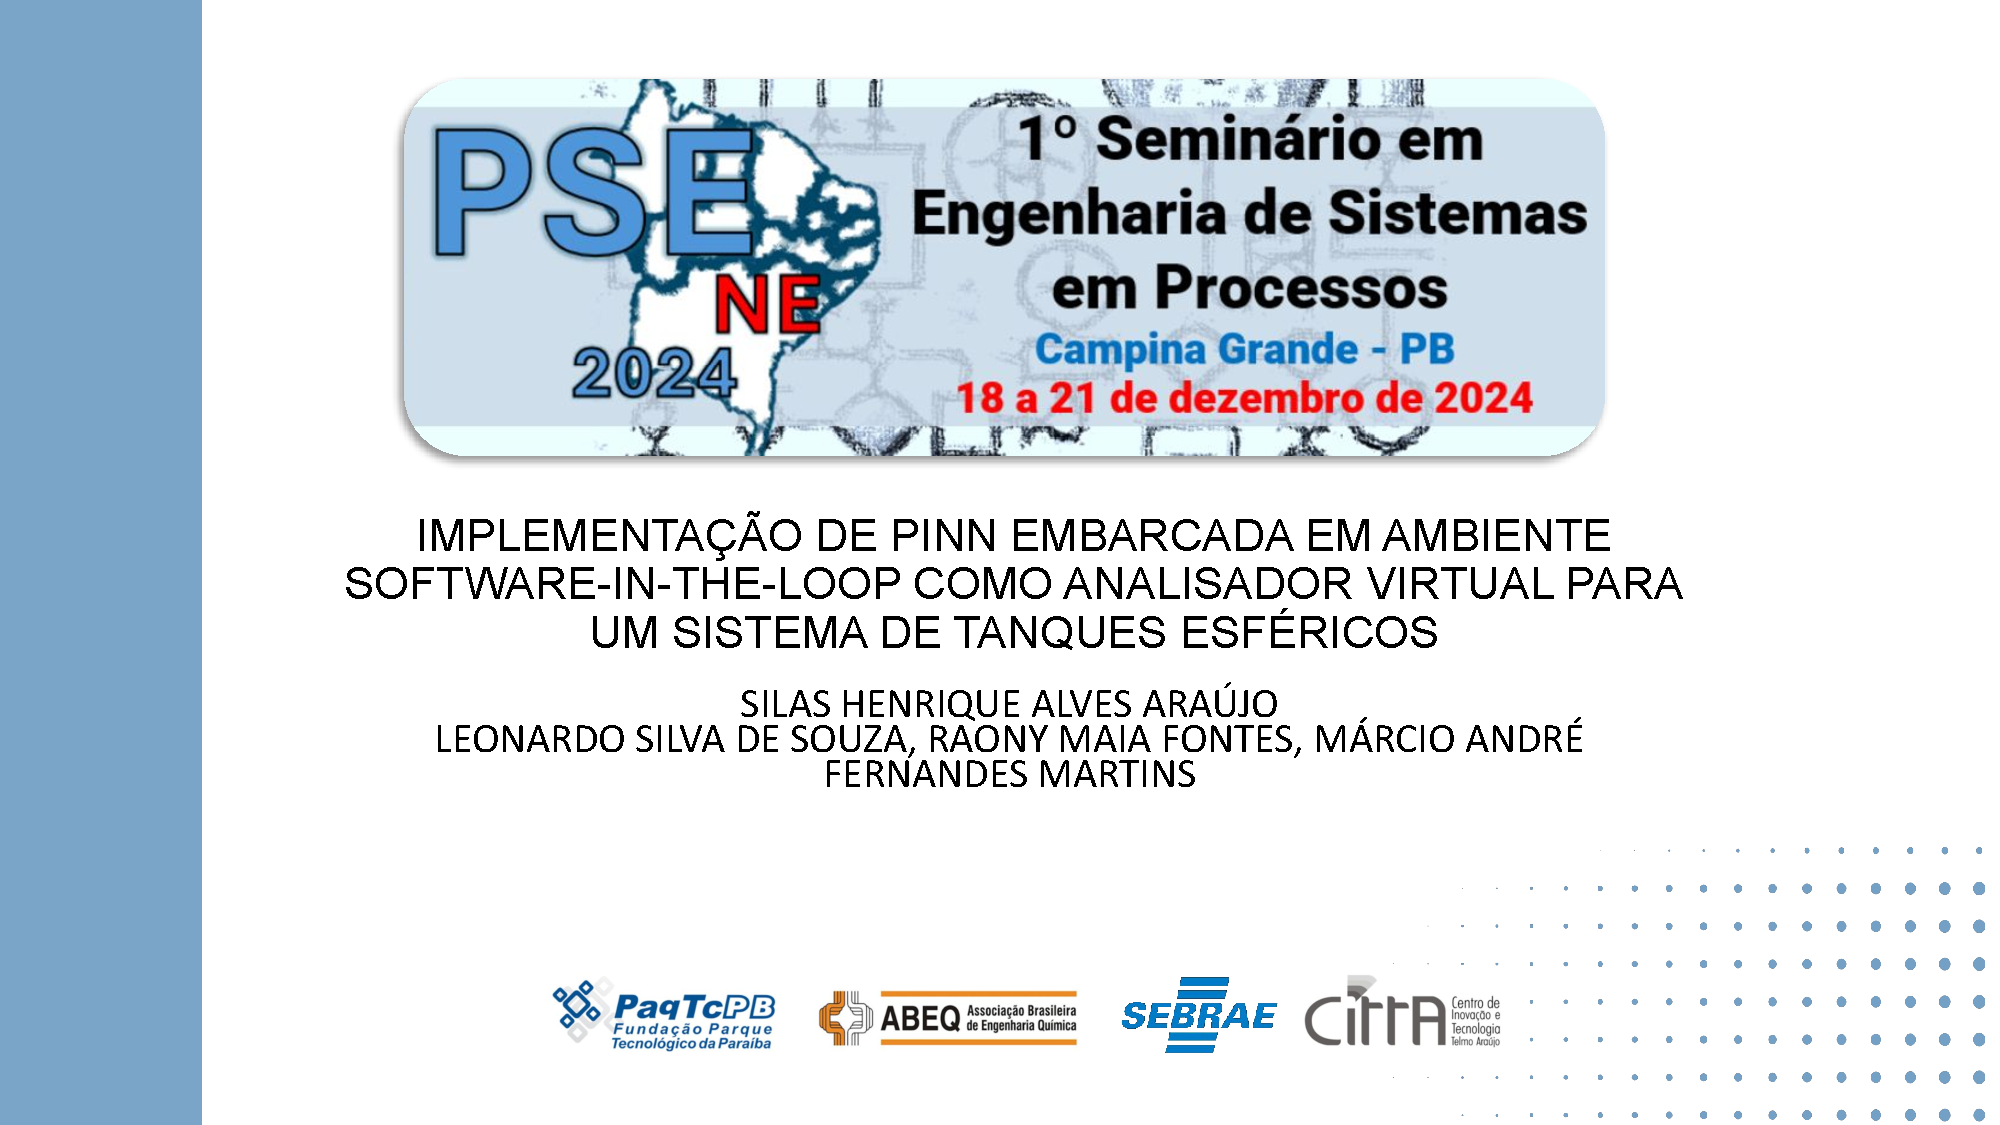
\includepdf[pages=1]{capa-pse.pdf}
}

\section{Introdução}

% Estruture como um funil, começando do mais geral para o mais especifico
%
% Simulação e controle
% Redes Neurais
% PINNs
% PIRNNs
% Deixe os tanques e software-in-the-loop para a metodologia
%
A simulação e o controle de processos são fundamentais para a indústria, desempenhando um papel essencial na eficiência e segurança dos processos. Através da simulação, é possível prever o comportamento de sistemas complexos sem a necessidade de intervenções físicas, o que permite identificar problemas, testar soluções e otimizar processos antes comprometer recursos físicos. O controle, por sua vez, assegura que os sistemas operem nos parâmetros estabelecidos, ajustando variáveis em tempo real para manter a estabilidade e a produtividade.

O trabalho conjunto entre simulação e controle é particularmente bem exemplificado no controle preditivo baseado em modelo (\textit{Model Predictive Control} — MPC), uma abordagem avançada que tem sido amplamente aplicada em indústrias de processos, como químicas e petroquímicas, desde o final da década de 1970 \citep{garcia_1989}. Nesse contexto, o uso de um modelo preciso do sistema é fundamental, por permitir prever a resposta futura do processo com base em seu estado atual e nas possíveis ações de controle.

Entretanto, na prática, a indústria enfrenta uma série de desafios práticos para implementação de um sistema assim. Por exemplo, é preciso que a resposta da simulação seja rápida o suficiente para fornecer previsões em tempo real para o controlador tomar decisões eficazes a cada novo ciclo. Dependendo do modelo utilizado, isso exige alto poder computacional, o que pode ser um problema para sistemas embarcados.% Além disso, a instrumentação do sistema deve ser precisa e confiável, com sensores que operem sincronizadamente e forneçam dados continuamente e sem atrasos.

% Um exemplo de sistema que pode apresentar esses desafios é a simulação e controle de nível em tanques esféricos. A dinâmica do nível de líquido nesses tanques é não linear devido à variação da área da seção transversal com a altura do líquido, o que significa que pequenas variações na vazão de entrada podem resultar em grandes mudanças na altura do líquido \citep{priya_2012}.

Uma abordagem diferente para esses problemas é o uso de redes neurais artificiais (\textit{Artificial Neural Networks} — ANNs). Elas são consideradas aproximadoras de funções universais \citep{csaji_2001} e têm o potencial de serem mais rápidas que os métodos numéricos convencionais por terem uma arquitetura baseada em operações simples e paralelizáveis. Em adendo, as ANNs podem ser treinadas integrando o modelo matemático do problema diretamente na função de custo penalizando previsões que violam as relações físicas conhecidas. Essa metodologia, denominada Rede Neural Fenomenologicamente Informada (\textit{Physics-Informed Neural Network} — PINN), é especialmente vantajosa para simular sistemas complexos e com poucos dados experimentais por combinar a flexibilidade das redes neurais com o rigor das equações diferenciais do problema físico \citep{raissi_2019}.

Uma variação dessa abordagem são as Redes Neurais Recorrentes Fenomenologicamente Informadas (\textit{Physics-Informed Recurrent Neural Networks} — PIRNNs), que aprimoram a capacidade de capturar dependências temporais, sendo particularmente úteis para prever a dinâmica de sistemas que evoluem temporalmente (\citep{zheng_2023}).

Essa pesquisa tem como objetivo explorar o uso de PIRNNs como uma alternativa aos métodos convencionais na simulação de sistemas dinâmicos. Especificamente, visa-se avaliar a redução no tempo de cômputo e a qualidade das previsões em comparação com os métodos numéricos tradicionais. Além disso, investiga-se a aplicabilidade dessas redes em sistemas embarcados, demonstrando a viabilidade de embarcar uma PIRNN em um microcontrolador de baixo custo.

\section{A PINN para Solução de EDOs}

\begin{frame}{Estrutura da Rede Neural utilizada}
  A rede neural utilizada consiste em 5 camadas com a função de ativação tangente hiperbólica $(\tanh)$ entre elas.

  \begin{itemize}
    \item Entrada: $x = t$;
    \item camada linear 1: 32 neurônios;
    \item camada linear 2: 32 neurônios;
    \item camada linear 3: 32 neurônios;
    \item camada linear 4: 32 neurônios;
    \item saída: $\mathbf{y} = [h_1, h_2]$.
  \end{itemize}

  Totalizando $32+32+32+32+2=130$ neurônios.
\end{frame}

\begin{frame}{Entendendo a função \textit{loss} utilizada}
  A função \textit{loss} utilizada combina o erro baseado nas equações diferenciais com o erro de dados simulados.

  \begin{equation}
    \mathcal{L} = w_1 \cdot \mathcal{L}_{\text{EDO}} + w_2 \cdot \mathcal{L}_{\text{IC}} + w_3 \cdot \mathcal{L}_{\text{data}}
  \end{equation}
  onde:
  \begin{itemize}
    \item $w_1, w_2, w_3$: pesos para o cálculo da \textit{loss};
    \item $\mathcal{L}_{\text{EDO}}$: erro das equações diferenciais;
    \item $\mathcal{L}_{\text{IC}}$: erro das condições iniciais;
    \item $\mathcal{L}_{\text{data}}$: erro dos dados;
    \item $\mathcal{L}$: erro total.
  \end{itemize}
\end{frame}

\begin{frame}
  \begin{figure}
    \centering
    \resizebox{\textwidth}{!}{% Graphic for TeX using PGF
% Title: /home/silas/Downloads/prh-35.1/LaTeX/common/figures/pinn-diagram.dia
% Creator: Dia v0.97+git
% CreationDate: Tue Dec  3 14:40:09 2024
% For: silas
% \usepackage{tikz}
% The following commands are not supported in PSTricks at present
% We define them conditionally, so when they are implemented,
% this pgf file will use them.
\ifx\du\undefined
  \newlength{\du}
\fi
\setlength{\du}{15\unitlength}
\begin{tikzpicture}[even odd rule]
  \pgftransformxscale{1.000000}
  \pgftransformyscale{-1.000000}
  \definecolor{dialinecolor}{rgb}{0.000000, 0.000000, 0.000000}
  \pgfsetstrokecolor{dialinecolor}
  \pgfsetstrokeopacity{1.000000}
  \definecolor{diafillcolor}{rgb}{1.000000, 1.000000, 1.000000}
  \pgfsetfillcolor{diafillcolor}
  \pgfsetfillopacity{1.000000}
  \pgfsetlinewidth{0.100000\du}
  \pgfsetdash{{0.300000\du}{0.300000\du}}{0\du}
  \pgfsetmiterjoin
  {\pgfsetcornersarced{\pgfpoint{0.500000\du}{0.500000\du}}\definecolor{diafillcolor}{rgb}{1.000000, 1.000000, 1.000000}
    \pgfsetfillcolor{diafillcolor}
    \pgfsetfillopacity{0.000000}
    \fill (34.000000\du,14.000000\du)--(34.000000\du,21.000000\du)--(38.000000\du,21.000000\du)--(38.000000\du,14.000000\du)--cycle;
  }{\pgfsetcornersarced{\pgfpoint{0.500000\du}{0.500000\du}}\definecolor{dialinecolor}{rgb}{0.000000, 0.000000, 0.000000}
    \pgfsetstrokecolor{dialinecolor}
    \pgfsetstrokeopacity{1.000000}
    \draw (34.000000\du,14.000000\du)--(34.000000\du,21.000000\du)--(38.000000\du,21.000000\du)--(38.000000\du,14.000000\du)--cycle;
  }% setfont left to latex
  \definecolor{dialinecolor}{rgb}{0.000000, 0.000000, 0.000000}
  \pgfsetstrokecolor{dialinecolor}
  \pgfsetstrokeopacity{1.000000}
  \definecolor{diafillcolor}{rgb}{0.000000, 0.000000, 0.000000}
  \pgfsetfillcolor{diafillcolor}
  \pgfsetfillopacity{1.000000}
  \node[anchor=base,inner sep=0pt, outer sep=0pt,color=dialinecolor] at (36.000000\du,17.691509\du){};
  \pgfsetlinewidth{0.100000\du}
  \pgfsetdash{{0.300000\du}{0.300000\du}}{0\du}
  \pgfsetmiterjoin
  {\pgfsetcornersarced{\pgfpoint{0.500000\du}{0.500000\du}}\definecolor{diafillcolor}{rgb}{1.000000, 1.000000, 1.000000}
    \pgfsetfillcolor{diafillcolor}
    \pgfsetfillopacity{0.000000}
    \fill (15.000000\du,14.000000\du)--(15.000000\du,27.000000\du)--(32.000000\du,27.000000\du)--(32.000000\du,14.000000\du)--cycle;
  }{\pgfsetcornersarced{\pgfpoint{0.500000\du}{0.500000\du}}\definecolor{dialinecolor}{rgb}{0.000000, 0.000000, 0.000000}
    \pgfsetstrokecolor{dialinecolor}
    \pgfsetstrokeopacity{1.000000}
    \draw (15.000000\du,14.000000\du)--(15.000000\du,27.000000\du)--(32.000000\du,27.000000\du)--(32.000000\du,14.000000\du)--cycle;
  }% setfont left to latex
  \definecolor{dialinecolor}{rgb}{0.000000, 0.000000, 0.000000}
  \pgfsetstrokecolor{dialinecolor}
  \pgfsetstrokeopacity{1.000000}
  \definecolor{diafillcolor}{rgb}{0.000000, 0.000000, 0.000000}
  \pgfsetfillcolor{diafillcolor}
  \pgfsetfillopacity{1.000000}
  \node[anchor=base,inner sep=0pt, outer sep=0pt,color=dialinecolor] at (23.500000\du,20.691509\du){};
  \pgfsetlinewidth{0.100000\du}
  \pgfsetdash{}{0pt}
  \pgfsetmiterjoin
  \definecolor{diafillcolor}{rgb}{1.000000, 1.000000, 1.000000}
  \pgfsetfillcolor{diafillcolor}
  \pgfsetfillopacity{1.000000}
  \pgfpathellipse{\pgfpoint{16.500000\du}{20.500000\du}}{\pgfpoint{1.000000\du}{0\du}}{\pgfpoint{0\du}{1.000000\du}}
  \pgfusepath{fill}
  \definecolor{dialinecolor}{rgb}{0.000000, 0.000000, 0.000000}
  \pgfsetstrokecolor{dialinecolor}
  \pgfsetstrokeopacity{1.000000}
  \pgfpathellipse{\pgfpoint{16.500000\du}{20.500000\du}}{\pgfpoint{1.000000\du}{0\du}}{\pgfpoint{0\du}{1.000000\du}}
  \pgfusepath{stroke}
  % setfont left to latex
  \definecolor{dialinecolor}{rgb}{0.000000, 0.000000, 0.000000}
  \pgfsetstrokecolor{dialinecolor}
  \pgfsetstrokeopacity{1.000000}
  \definecolor{diafillcolor}{rgb}{0.000000, 0.000000, 0.000000}
  \pgfsetfillcolor{diafillcolor}
  \pgfsetfillopacity{1.000000}
  \node[anchor=base,inner sep=0pt, outer sep=0pt,color=dialinecolor] at (16.500000\du,20.694063\du){};
  \pgfsetlinewidth{0.100000\du}
  \pgfsetdash{}{0pt}
  \pgfsetmiterjoin
  \definecolor{diafillcolor}{rgb}{1.000000, 1.000000, 1.000000}
  \pgfsetfillcolor{diafillcolor}
  \pgfsetfillopacity{1.000000}
  \pgfpathellipse{\pgfpoint{21.000000\du}{16.000000\du}}{\pgfpoint{1.000000\du}{0\du}}{\pgfpoint{0\du}{1.000000\du}}
  \pgfusepath{fill}
  \definecolor{dialinecolor}{rgb}{0.000000, 0.000000, 0.000000}
  \pgfsetstrokecolor{dialinecolor}
  \pgfsetstrokeopacity{1.000000}
  \pgfpathellipse{\pgfpoint{21.000000\du}{16.000000\du}}{\pgfpoint{1.000000\du}{0\du}}{\pgfpoint{0\du}{1.000000\du}}
  \pgfusepath{stroke}
  % setfont left to latex
  \definecolor{dialinecolor}{rgb}{0.000000, 0.000000, 0.000000}
  \pgfsetstrokecolor{dialinecolor}
  \pgfsetstrokeopacity{1.000000}
  \definecolor{diafillcolor}{rgb}{0.000000, 0.000000, 0.000000}
  \pgfsetfillcolor{diafillcolor}
  \pgfsetfillopacity{1.000000}
  \node[anchor=base,inner sep=0pt, outer sep=0pt,color=dialinecolor] at (21.000000\du,16.194063\du){};
  \pgfsetlinewidth{0.100000\du}
  \pgfsetdash{}{0pt}
  \pgfsetmiterjoin
  \definecolor{diafillcolor}{rgb}{1.000000, 1.000000, 1.000000}
  \pgfsetfillcolor{diafillcolor}
  \pgfsetfillopacity{1.000000}
  \pgfpathellipse{\pgfpoint{21.000000\du}{19.000000\du}}{\pgfpoint{1.000000\du}{0\du}}{\pgfpoint{0\du}{1.000000\du}}
  \pgfusepath{fill}
  \definecolor{dialinecolor}{rgb}{0.000000, 0.000000, 0.000000}
  \pgfsetstrokecolor{dialinecolor}
  \pgfsetstrokeopacity{1.000000}
  \pgfpathellipse{\pgfpoint{21.000000\du}{19.000000\du}}{\pgfpoint{1.000000\du}{0\du}}{\pgfpoint{0\du}{1.000000\du}}
  \pgfusepath{stroke}
  % setfont left to latex
  \definecolor{dialinecolor}{rgb}{0.000000, 0.000000, 0.000000}
  \pgfsetstrokecolor{dialinecolor}
  \pgfsetstrokeopacity{1.000000}
  \definecolor{diafillcolor}{rgb}{0.000000, 0.000000, 0.000000}
  \pgfsetfillcolor{diafillcolor}
  \pgfsetfillopacity{1.000000}
  \node[anchor=base,inner sep=0pt, outer sep=0pt,color=dialinecolor] at (21.000000\du,19.194063\du){};
  \pgfsetlinewidth{0.100000\du}
  \pgfsetdash{}{0pt}
  \pgfsetmiterjoin
  \definecolor{diafillcolor}{rgb}{1.000000, 1.000000, 1.000000}
  \pgfsetfillcolor{diafillcolor}
  \pgfsetfillopacity{1.000000}
  \pgfpathellipse{\pgfpoint{21.000000\du}{25.000000\du}}{\pgfpoint{1.000000\du}{0\du}}{\pgfpoint{0\du}{1.000000\du}}
  \pgfusepath{fill}
  \definecolor{dialinecolor}{rgb}{0.000000, 0.000000, 0.000000}
  \pgfsetstrokecolor{dialinecolor}
  \pgfsetstrokeopacity{1.000000}
  \pgfpathellipse{\pgfpoint{21.000000\du}{25.000000\du}}{\pgfpoint{1.000000\du}{0\du}}{\pgfpoint{0\du}{1.000000\du}}
  \pgfusepath{stroke}
  % setfont left to latex
  \definecolor{dialinecolor}{rgb}{0.000000, 0.000000, 0.000000}
  \pgfsetstrokecolor{dialinecolor}
  \pgfsetstrokeopacity{1.000000}
  \definecolor{diafillcolor}{rgb}{0.000000, 0.000000, 0.000000}
  \pgfsetfillcolor{diafillcolor}
  \pgfsetfillopacity{1.000000}
  \node[anchor=base,inner sep=0pt, outer sep=0pt,color=dialinecolor] at (21.000000\du,25.194063\du){};
  \pgfsetlinewidth{0.100000\du}
  \pgfsetdash{}{0pt}
  \pgfsetmiterjoin
  \definecolor{diafillcolor}{rgb}{1.000000, 1.000000, 1.000000}
  \pgfsetfillcolor{diafillcolor}
  \pgfsetfillopacity{1.000000}
  \pgfpathellipse{\pgfpoint{25.500000\du}{16.000000\du}}{\pgfpoint{1.000000\du}{0\du}}{\pgfpoint{0\du}{1.000000\du}}
  \pgfusepath{fill}
  \definecolor{dialinecolor}{rgb}{0.000000, 0.000000, 0.000000}
  \pgfsetstrokecolor{dialinecolor}
  \pgfsetstrokeopacity{1.000000}
  \pgfpathellipse{\pgfpoint{25.500000\du}{16.000000\du}}{\pgfpoint{1.000000\du}{0\du}}{\pgfpoint{0\du}{1.000000\du}}
  \pgfusepath{stroke}
  % setfont left to latex
  \definecolor{dialinecolor}{rgb}{0.000000, 0.000000, 0.000000}
  \pgfsetstrokecolor{dialinecolor}
  \pgfsetstrokeopacity{1.000000}
  \definecolor{diafillcolor}{rgb}{0.000000, 0.000000, 0.000000}
  \pgfsetfillcolor{diafillcolor}
  \pgfsetfillopacity{1.000000}
  \node[anchor=base,inner sep=0pt, outer sep=0pt,color=dialinecolor] at (25.500000\du,16.194063\du){};
  \pgfsetlinewidth{0.100000\du}
  \pgfsetdash{}{0pt}
  \pgfsetmiterjoin
  \definecolor{diafillcolor}{rgb}{1.000000, 1.000000, 1.000000}
  \pgfsetfillcolor{diafillcolor}
  \pgfsetfillopacity{1.000000}
  \pgfpathellipse{\pgfpoint{25.500000\du}{19.000000\du}}{\pgfpoint{1.000000\du}{0\du}}{\pgfpoint{0\du}{1.000000\du}}
  \pgfusepath{fill}
  \definecolor{dialinecolor}{rgb}{0.000000, 0.000000, 0.000000}
  \pgfsetstrokecolor{dialinecolor}
  \pgfsetstrokeopacity{1.000000}
  \pgfpathellipse{\pgfpoint{25.500000\du}{19.000000\du}}{\pgfpoint{1.000000\du}{0\du}}{\pgfpoint{0\du}{1.000000\du}}
  \pgfusepath{stroke}
  % setfont left to latex
  \definecolor{dialinecolor}{rgb}{0.000000, 0.000000, 0.000000}
  \pgfsetstrokecolor{dialinecolor}
  \pgfsetstrokeopacity{1.000000}
  \definecolor{diafillcolor}{rgb}{0.000000, 0.000000, 0.000000}
  \pgfsetfillcolor{diafillcolor}
  \pgfsetfillopacity{1.000000}
  \node[anchor=base,inner sep=0pt, outer sep=0pt,color=dialinecolor] at (25.500000\du,19.194063\du){};
  \pgfsetlinewidth{0.100000\du}
  \pgfsetdash{}{0pt}
  \pgfsetmiterjoin
  \definecolor{diafillcolor}{rgb}{1.000000, 1.000000, 1.000000}
  \pgfsetfillcolor{diafillcolor}
  \pgfsetfillopacity{1.000000}
  \pgfpathellipse{\pgfpoint{25.500000\du}{25.000000\du}}{\pgfpoint{1.000000\du}{0\du}}{\pgfpoint{0\du}{1.000000\du}}
  \pgfusepath{fill}
  \definecolor{dialinecolor}{rgb}{0.000000, 0.000000, 0.000000}
  \pgfsetstrokecolor{dialinecolor}
  \pgfsetstrokeopacity{1.000000}
  \pgfpathellipse{\pgfpoint{25.500000\du}{25.000000\du}}{\pgfpoint{1.000000\du}{0\du}}{\pgfpoint{0\du}{1.000000\du}}
  \pgfusepath{stroke}
  % setfont left to latex
  \definecolor{dialinecolor}{rgb}{0.000000, 0.000000, 0.000000}
  \pgfsetstrokecolor{dialinecolor}
  \pgfsetstrokeopacity{1.000000}
  \definecolor{diafillcolor}{rgb}{0.000000, 0.000000, 0.000000}
  \pgfsetfillcolor{diafillcolor}
  \pgfsetfillopacity{1.000000}
  \node[anchor=base,inner sep=0pt, outer sep=0pt,color=dialinecolor] at (25.500000\du,25.194063\du){};
  \pgfsetlinewidth{0.100000\du}
  \pgfsetdash{}{0pt}
  \pgfsetmiterjoin
  \definecolor{diafillcolor}{rgb}{1.000000, 1.000000, 1.000000}
  \pgfsetfillcolor{diafillcolor}
  \pgfsetfillopacity{1.000000}
  \pgfpathellipse{\pgfpoint{30.000000\du}{19.000000\du}}{\pgfpoint{1.000000\du}{0\du}}{\pgfpoint{0\du}{1.000000\du}}
  \pgfusepath{fill}
  \definecolor{dialinecolor}{rgb}{0.000000, 0.000000, 0.000000}
  \pgfsetstrokecolor{dialinecolor}
  \pgfsetstrokeopacity{1.000000}
  \pgfpathellipse{\pgfpoint{30.000000\du}{19.000000\du}}{\pgfpoint{1.000000\du}{0\du}}{\pgfpoint{0\du}{1.000000\du}}
  \pgfusepath{stroke}
  % setfont left to latex
  \definecolor{dialinecolor}{rgb}{0.000000, 0.000000, 0.000000}
  \pgfsetstrokecolor{dialinecolor}
  \pgfsetstrokeopacity{1.000000}
  \definecolor{diafillcolor}{rgb}{0.000000, 0.000000, 0.000000}
  \pgfsetfillcolor{diafillcolor}
  \pgfsetfillopacity{1.000000}
  \node[anchor=base,inner sep=0pt, outer sep=0pt,color=dialinecolor] at (30.000000\du,19.194063\du){};
  \pgfsetlinewidth{0.100000\du}
  \pgfsetdash{}{0pt}
  \pgfsetmiterjoin
  \definecolor{diafillcolor}{rgb}{1.000000, 1.000000, 1.000000}
  \pgfsetfillcolor{diafillcolor}
  \pgfsetfillopacity{1.000000}
  \pgfpathellipse{\pgfpoint{30.000000\du}{22.000000\du}}{\pgfpoint{1.000000\du}{0\du}}{\pgfpoint{0\du}{1.000000\du}}
  \pgfusepath{fill}
  \definecolor{dialinecolor}{rgb}{0.000000, 0.000000, 0.000000}
  \pgfsetstrokecolor{dialinecolor}
  \pgfsetstrokeopacity{1.000000}
  \pgfpathellipse{\pgfpoint{30.000000\du}{22.000000\du}}{\pgfpoint{1.000000\du}{0\du}}{\pgfpoint{0\du}{1.000000\du}}
  \pgfusepath{stroke}
  % setfont left to latex
  \definecolor{dialinecolor}{rgb}{0.000000, 0.000000, 0.000000}
  \pgfsetstrokecolor{dialinecolor}
  \pgfsetstrokeopacity{1.000000}
  \definecolor{diafillcolor}{rgb}{0.000000, 0.000000, 0.000000}
  \pgfsetfillcolor{diafillcolor}
  \pgfsetfillopacity{1.000000}
  \node[anchor=base,inner sep=0pt, outer sep=0pt,color=dialinecolor] at (30.000000\du,22.194063\du){};
  \pgfsetlinewidth{0.100000\du}
  \pgfsetdash{}{0pt}
  \pgfsetbuttcap
  {
    \definecolor{diafillcolor}{rgb}{0.000000, 0.000000, 0.000000}
    \pgfsetfillcolor{diafillcolor}
    \pgfsetfillopacity{1.000000}
    % was here!!!
    \pgfsetarrowsend{stealth}
    \definecolor{dialinecolor}{rgb}{0.000000, 0.000000, 0.000000}
    \pgfsetstrokecolor{dialinecolor}
    \pgfsetstrokeopacity{1.000000}
    \draw (17.500000\du,20.500000\du)--(20.000000\du,19.000000\du);
  }
  \pgfsetlinewidth{0.100000\du}
  \pgfsetdash{}{0pt}
  \pgfsetbuttcap
  {
    \definecolor{diafillcolor}{rgb}{0.000000, 0.000000, 0.000000}
    \pgfsetfillcolor{diafillcolor}
    \pgfsetfillopacity{1.000000}
    % was here!!!
    \pgfsetarrowsend{stealth}
    \definecolor{dialinecolor}{rgb}{0.000000, 0.000000, 0.000000}
    \pgfsetstrokecolor{dialinecolor}
    \pgfsetstrokeopacity{1.000000}
    \draw (17.500000\du,20.500000\du)--(20.000000\du,25.000000\du);
  }
  \pgfsetlinewidth{0.100000\du}
  \pgfsetdash{}{0pt}
  \pgfsetbuttcap
  {
    \definecolor{diafillcolor}{rgb}{0.000000, 0.000000, 0.000000}
    \pgfsetfillcolor{diafillcolor}
    \pgfsetfillopacity{1.000000}
    % was here!!!
    \pgfsetarrowsend{stealth}
    \definecolor{dialinecolor}{rgb}{0.000000, 0.000000, 0.000000}
    \pgfsetstrokecolor{dialinecolor}
    \pgfsetstrokeopacity{1.000000}
    \draw (17.500000\du,20.500000\du)--(20.000000\du,16.000000\du);
  }
  \pgfsetlinewidth{0.100000\du}
  \pgfsetdash{}{0pt}
  \pgfsetbuttcap
  {
    \definecolor{diafillcolor}{rgb}{0.000000, 0.000000, 0.000000}
    \pgfsetfillcolor{diafillcolor}
    \pgfsetfillopacity{1.000000}
    % was here!!!
    \pgfsetarrowsend{stealth}
    \definecolor{dialinecolor}{rgb}{0.000000, 0.000000, 0.000000}
    \pgfsetstrokecolor{dialinecolor}
    \pgfsetstrokeopacity{1.000000}
    \draw (26.500000\du,16.000000\du)--(29.000000\du,19.000000\du);
  }
  \pgfsetlinewidth{0.100000\du}
  \pgfsetdash{}{0pt}
  \pgfsetbuttcap
  {
    \definecolor{diafillcolor}{rgb}{0.000000, 0.000000, 0.000000}
    \pgfsetfillcolor{diafillcolor}
    \pgfsetfillopacity{1.000000}
    % was here!!!
    \pgfsetarrowsend{stealth}
    \definecolor{dialinecolor}{rgb}{0.000000, 0.000000, 0.000000}
    \pgfsetstrokecolor{dialinecolor}
    \pgfsetstrokeopacity{1.000000}
    \draw (26.500000\du,16.000000\du)--(29.000000\du,22.000000\du);
  }
  \pgfsetlinewidth{0.100000\du}
  \pgfsetdash{}{0pt}
  \pgfsetbuttcap
  {
    \definecolor{diafillcolor}{rgb}{0.000000, 0.000000, 0.000000}
    \pgfsetfillcolor{diafillcolor}
    \pgfsetfillopacity{1.000000}
    % was here!!!
    \pgfsetarrowsend{stealth}
    \definecolor{dialinecolor}{rgb}{0.000000, 0.000000, 0.000000}
    \pgfsetstrokecolor{dialinecolor}
    \pgfsetstrokeopacity{1.000000}
    \draw (26.500000\du,19.000000\du)--(29.000000\du,19.000000\du);
  }
  \pgfsetlinewidth{0.100000\du}
  \pgfsetdash{}{0pt}
  \pgfsetbuttcap
  {
    \definecolor{diafillcolor}{rgb}{0.000000, 0.000000, 0.000000}
    \pgfsetfillcolor{diafillcolor}
    \pgfsetfillopacity{1.000000}
    % was here!!!
    \pgfsetarrowsend{stealth}
    \definecolor{dialinecolor}{rgb}{0.000000, 0.000000, 0.000000}
    \pgfsetstrokecolor{dialinecolor}
    \pgfsetstrokeopacity{1.000000}
    \draw (26.500000\du,19.000000\du)--(29.000000\du,22.000000\du);
  }
  \pgfsetlinewidth{0.100000\du}
  \pgfsetdash{}{0pt}
  \pgfsetbuttcap
  {
    \definecolor{diafillcolor}{rgb}{0.000000, 0.000000, 0.000000}
    \pgfsetfillcolor{diafillcolor}
    \pgfsetfillopacity{1.000000}
    % was here!!!
    \pgfsetarrowsend{stealth}
    \definecolor{dialinecolor}{rgb}{0.000000, 0.000000, 0.000000}
    \pgfsetstrokecolor{dialinecolor}
    \pgfsetstrokeopacity{1.000000}
    \draw (26.500000\du,25.000000\du)--(29.000000\du,22.000000\du);
  }
  \pgfsetlinewidth{0.100000\du}
  \pgfsetdash{}{0pt}
  \pgfsetbuttcap
  {
    \definecolor{diafillcolor}{rgb}{0.000000, 0.000000, 0.000000}
    \pgfsetfillcolor{diafillcolor}
    \pgfsetfillopacity{1.000000}
    % was here!!!
    \pgfsetarrowsend{stealth}
    \definecolor{dialinecolor}{rgb}{0.000000, 0.000000, 0.000000}
    \pgfsetstrokecolor{dialinecolor}
    \pgfsetstrokeopacity{1.000000}
    \draw (26.500000\du,25.000000\du)--(29.000000\du,19.000000\du);
  }
  \pgfsetlinewidth{0.100000\du}
  \pgfsetdash{}{0pt}
  \pgfsetbuttcap
  {
    \definecolor{diafillcolor}{rgb}{0.000000, 0.000000, 0.000000}
    \pgfsetfillcolor{diafillcolor}
    \pgfsetfillopacity{1.000000}
    % was here!!!
    \pgfsetarrowsend{stealth}
    \definecolor{dialinecolor}{rgb}{0.000000, 0.000000, 0.000000}
    \pgfsetstrokecolor{dialinecolor}
    \pgfsetstrokeopacity{1.000000}
    \draw (22.000000\du,25.000000\du)--(24.500000\du,25.000000\du);
  }
  \pgfsetlinewidth{0.100000\du}
  \pgfsetdash{}{0pt}
  \pgfsetbuttcap
  {
    \definecolor{diafillcolor}{rgb}{0.000000, 0.000000, 0.000000}
    \pgfsetfillcolor{diafillcolor}
    \pgfsetfillopacity{1.000000}
    % was here!!!
    \pgfsetarrowsend{stealth}
    \definecolor{dialinecolor}{rgb}{0.000000, 0.000000, 0.000000}
    \pgfsetstrokecolor{dialinecolor}
    \pgfsetstrokeopacity{1.000000}
    \draw (22.000000\du,16.000000\du)--(24.500000\du,16.000000\du);
  }
  \pgfsetlinewidth{0.100000\du}
  \pgfsetdash{}{0pt}
  \pgfsetbuttcap
  {
    \definecolor{diafillcolor}{rgb}{0.000000, 0.000000, 0.000000}
    \pgfsetfillcolor{diafillcolor}
    \pgfsetfillopacity{1.000000}
    % was here!!!
    \pgfsetarrowsend{stealth}
    \definecolor{dialinecolor}{rgb}{0.000000, 0.000000, 0.000000}
    \pgfsetstrokecolor{dialinecolor}
    \pgfsetstrokeopacity{1.000000}
    \draw (22.000000\du,16.000000\du)--(24.500000\du,19.000000\du);
  }
  \pgfsetlinewidth{0.100000\du}
  \pgfsetdash{}{0pt}
  \pgfsetbuttcap
  {
    \definecolor{diafillcolor}{rgb}{0.000000, 0.000000, 0.000000}
    \pgfsetfillcolor{diafillcolor}
    \pgfsetfillopacity{1.000000}
    % was here!!!
    \pgfsetarrowsend{stealth}
    \definecolor{dialinecolor}{rgb}{0.000000, 0.000000, 0.000000}
    \pgfsetstrokecolor{dialinecolor}
    \pgfsetstrokeopacity{1.000000}
    \draw (22.000000\du,16.000000\du)--(24.500000\du,25.000000\du);
  }
  \pgfsetlinewidth{0.100000\du}
  \pgfsetdash{}{0pt}
  \pgfsetbuttcap
  {
    \definecolor{diafillcolor}{rgb}{0.000000, 0.000000, 0.000000}
    \pgfsetfillcolor{diafillcolor}
    \pgfsetfillopacity{1.000000}
    % was here!!!
    \pgfsetarrowsend{stealth}
    \definecolor{dialinecolor}{rgb}{0.000000, 0.000000, 0.000000}
    \pgfsetstrokecolor{dialinecolor}
    \pgfsetstrokeopacity{1.000000}
    \draw (22.000000\du,19.000000\du)--(24.500000\du,16.000000\du);
  }
  \pgfsetlinewidth{0.100000\du}
  \pgfsetdash{}{0pt}
  \pgfsetbuttcap
  {
    \definecolor{diafillcolor}{rgb}{0.000000, 0.000000, 0.000000}
    \pgfsetfillcolor{diafillcolor}
    \pgfsetfillopacity{1.000000}
    % was here!!!
    \pgfsetarrowsend{stealth}
    \definecolor{dialinecolor}{rgb}{0.000000, 0.000000, 0.000000}
    \pgfsetstrokecolor{dialinecolor}
    \pgfsetstrokeopacity{1.000000}
    \draw (22.000000\du,19.000000\du)--(24.500000\du,19.000000\du);
  }
  \pgfsetlinewidth{0.100000\du}
  \pgfsetdash{}{0pt}
  \pgfsetbuttcap
  {
    \definecolor{diafillcolor}{rgb}{0.000000, 0.000000, 0.000000}
    \pgfsetfillcolor{diafillcolor}
    \pgfsetfillopacity{1.000000}
    % was here!!!
    \pgfsetarrowsend{stealth}
    \definecolor{dialinecolor}{rgb}{0.000000, 0.000000, 0.000000}
    \pgfsetstrokecolor{dialinecolor}
    \pgfsetstrokeopacity{1.000000}
    \draw (22.000000\du,19.000000\du)--(24.500000\du,25.000000\du);
  }
  \pgfsetlinewidth{0.100000\du}
  \pgfsetdash{}{0pt}
  \pgfsetbuttcap
  {
    \definecolor{diafillcolor}{rgb}{0.000000, 0.000000, 0.000000}
    \pgfsetfillcolor{diafillcolor}
    \pgfsetfillopacity{1.000000}
    % was here!!!
    \pgfsetarrowsend{stealth}
    \definecolor{dialinecolor}{rgb}{0.000000, 0.000000, 0.000000}
    \pgfsetstrokecolor{dialinecolor}
    \pgfsetstrokeopacity{1.000000}
    \draw (22.000000\du,25.000000\du)--(24.500000\du,19.000000\du);
  }
  \pgfsetlinewidth{0.100000\du}
  \pgfsetdash{}{0pt}
  \pgfsetbuttcap
  {
    \definecolor{diafillcolor}{rgb}{0.000000, 0.000000, 0.000000}
    \pgfsetfillcolor{diafillcolor}
    \pgfsetfillopacity{1.000000}
    % was here!!!
    \pgfsetarrowsend{stealth}
    \definecolor{dialinecolor}{rgb}{0.000000, 0.000000, 0.000000}
    \pgfsetstrokecolor{dialinecolor}
    \pgfsetstrokeopacity{1.000000}
    \draw (22.000000\du,25.000000\du)--(24.500000\du,16.000000\du);
  }
  % setfont left to latex
  \definecolor{dialinecolor}{rgb}{0.000000, 0.000000, 0.000000}
  \pgfsetstrokecolor{dialinecolor}
  \pgfsetstrokeopacity{1.000000}
  \definecolor{diafillcolor}{rgb}{0.000000, 0.000000, 0.000000}
  \pgfsetfillcolor{diafillcolor}
  \pgfsetfillopacity{1.000000}
  \node[anchor=base,inner sep=0pt, outer sep=0pt,color=dialinecolor] at (21.000000\du,21.421563\du){.};
  % setfont left to latex
  \definecolor{dialinecolor}{rgb}{0.000000, 0.000000, 0.000000}
  \pgfsetstrokecolor{dialinecolor}
  \pgfsetstrokeopacity{1.000000}
  \definecolor{diafillcolor}{rgb}{0.000000, 0.000000, 0.000000}
  \pgfsetfillcolor{diafillcolor}
  \pgfsetfillopacity{1.000000}
  \node[anchor=base,inner sep=0pt, outer sep=0pt,color=dialinecolor] at (21.000000\du,22.221563\du){.};
  % setfont left to latex
  \definecolor{dialinecolor}{rgb}{0.000000, 0.000000, 0.000000}
  \pgfsetstrokecolor{dialinecolor}
  \pgfsetstrokeopacity{1.000000}
  \definecolor{diafillcolor}{rgb}{0.000000, 0.000000, 0.000000}
  \pgfsetfillcolor{diafillcolor}
  \pgfsetfillopacity{1.000000}
  \node[anchor=base,inner sep=0pt, outer sep=0pt,color=dialinecolor] at (21.000000\du,23.021563\du){.};
  % setfont left to latex
  \definecolor{dialinecolor}{rgb}{0.000000, 0.000000, 0.000000}
  \pgfsetstrokecolor{dialinecolor}
  \pgfsetstrokeopacity{1.000000}
  \definecolor{diafillcolor}{rgb}{0.000000, 0.000000, 0.000000}
  \pgfsetfillcolor{diafillcolor}
  \pgfsetfillopacity{1.000000}
  \node[anchor=base,inner sep=0pt, outer sep=0pt,color=dialinecolor] at (25.500000\du,21.421563\du){.};
  % setfont left to latex
  \definecolor{dialinecolor}{rgb}{0.000000, 0.000000, 0.000000}
  \pgfsetstrokecolor{dialinecolor}
  \pgfsetstrokeopacity{1.000000}
  \definecolor{diafillcolor}{rgb}{0.000000, 0.000000, 0.000000}
  \pgfsetfillcolor{diafillcolor}
  \pgfsetfillopacity{1.000000}
  \node[anchor=base,inner sep=0pt, outer sep=0pt,color=dialinecolor] at (25.500000\du,22.221563\du){.};
  % setfont left to latex
  \definecolor{dialinecolor}{rgb}{0.000000, 0.000000, 0.000000}
  \pgfsetstrokecolor{dialinecolor}
  \pgfsetstrokeopacity{1.000000}
  \definecolor{diafillcolor}{rgb}{0.000000, 0.000000, 0.000000}
  \pgfsetfillcolor{diafillcolor}
  \pgfsetfillopacity{1.000000}
  \node[anchor=base,inner sep=0pt, outer sep=0pt,color=dialinecolor] at (25.500000\du,23.021563\du){.};
  \pgfsetlinewidth{0.100000\du}
  \pgfsetdash{}{0pt}
  \pgfsetmiterjoin
  \definecolor{diafillcolor}{rgb}{1.000000, 1.000000, 1.000000}
  \pgfsetfillcolor{diafillcolor}
  \pgfsetfillopacity{1.000000}
  \pgfpathellipse{\pgfpoint{36.000000\du}{16.000000\du}}{\pgfpoint{1.000000\du}{0\du}}{\pgfpoint{0\du}{1.000000\du}}
  \pgfusepath{fill}
  \definecolor{dialinecolor}{rgb}{0.000000, 0.000000, 0.000000}
  \pgfsetstrokecolor{dialinecolor}
  \pgfsetstrokeopacity{1.000000}
  \pgfpathellipse{\pgfpoint{36.000000\du}{16.000000\du}}{\pgfpoint{1.000000\du}{0\du}}{\pgfpoint{0\du}{1.000000\du}}
  \pgfusepath{stroke}
  % setfont left to latex
  \definecolor{dialinecolor}{rgb}{0.000000, 0.000000, 0.000000}
  \pgfsetstrokecolor{dialinecolor}
  \pgfsetstrokeopacity{1.000000}
  \definecolor{diafillcolor}{rgb}{0.000000, 0.000000, 0.000000}
  \pgfsetfillcolor{diafillcolor}
  \pgfsetfillopacity{1.000000}
  \node[anchor=base,inner sep=0pt, outer sep=0pt,color=dialinecolor] at (36.000000\du,16.128361\du){};
  \pgfsetlinewidth{0.100000\du}
  \pgfsetdash{}{0pt}
  \pgfsetmiterjoin
  {\pgfsetcornersarced{\pgfpoint{0.000000\du}{0.000000\du}}\definecolor{diafillcolor}{rgb}{1.000000, 1.000000, 1.000000}
    \pgfsetfillcolor{diafillcolor}
    \pgfsetfillopacity{1.000000}
    \fill (40.000000\du,21.500000\du)--(40.000000\du,23.500000\du)--(47.500000\du,23.500000\du)--(47.500000\du,21.500000\du)--cycle;
  }{\pgfsetcornersarced{\pgfpoint{0.000000\du}{0.000000\du}}\definecolor{dialinecolor}{rgb}{0.000000, 0.000000, 0.000000}
    \pgfsetstrokecolor{dialinecolor}
    \pgfsetstrokeopacity{1.000000}
    \draw (40.000000\du,21.500000\du)--(40.000000\du,23.500000\du)--(47.500000\du,23.500000\du)--(47.500000\du,21.500000\du)--cycle;
  }% setfont left to latex
  \definecolor{dialinecolor}{rgb}{0.000000, 0.000000, 0.000000}
  \pgfsetstrokecolor{dialinecolor}
  \pgfsetstrokeopacity{1.000000}
  \definecolor{diafillcolor}{rgb}{0.000000, 0.000000, 0.000000}
  \pgfsetfillcolor{diafillcolor}
  \pgfsetfillopacity{1.000000}
  \node[anchor=base,inner sep=0pt, outer sep=0pt,color=dialinecolor] at (43.750000\du,22.694063\du){Loss};
  % setfont left to latex
  \definecolor{dialinecolor}{rgb}{0.000000, 0.000000, 0.000000}
  \pgfsetstrokecolor{dialinecolor}
  \pgfsetstrokeopacity{1.000000}
  \definecolor{diafillcolor}{rgb}{0.000000, 0.000000, 0.000000}
  \pgfsetfillcolor{diafillcolor}
  \pgfsetfillopacity{1.000000}
  \node[anchor=base,inner sep=0pt, outer sep=0pt,color=dialinecolor] at (16.500000\du,20.712250\du){$t$};
  % setfont left to latex
  \definecolor{dialinecolor}{rgb}{0.000000, 0.000000, 0.000000}
  \pgfsetstrokecolor{dialinecolor}
  \pgfsetstrokeopacity{1.000000}
  \definecolor{diafillcolor}{rgb}{0.000000, 0.000000, 0.000000}
  \pgfsetfillcolor{diafillcolor}
  \pgfsetfillopacity{1.000000}
  \node[anchor=base,inner sep=0pt, outer sep=0pt,color=dialinecolor] at (21.000000\du,16.212250\du){$f$};
  % setfont left to latex
  \definecolor{dialinecolor}{rgb}{0.000000, 0.000000, 0.000000}
  \pgfsetstrokecolor{dialinecolor}
  \pgfsetstrokeopacity{1.000000}
  \definecolor{diafillcolor}{rgb}{0.000000, 0.000000, 0.000000}
  \pgfsetfillcolor{diafillcolor}
  \pgfsetfillopacity{1.000000}
  \node[anchor=base,inner sep=0pt, outer sep=0pt,color=dialinecolor] at (21.000000\du,19.212250\du){$f$};
  % setfont left to latex
  \definecolor{dialinecolor}{rgb}{0.000000, 0.000000, 0.000000}
  \pgfsetstrokecolor{dialinecolor}
  \pgfsetstrokeopacity{1.000000}
  \definecolor{diafillcolor}{rgb}{0.000000, 0.000000, 0.000000}
  \pgfsetfillcolor{diafillcolor}
  \pgfsetfillopacity{1.000000}
  \node[anchor=base,inner sep=0pt, outer sep=0pt,color=dialinecolor] at (21.000000\du,25.212250\du){$f$};
  % setfont left to latex
  \definecolor{dialinecolor}{rgb}{0.000000, 0.000000, 0.000000}
  \pgfsetstrokecolor{dialinecolor}
  \pgfsetstrokeopacity{1.000000}
  \definecolor{diafillcolor}{rgb}{0.000000, 0.000000, 0.000000}
  \pgfsetfillcolor{diafillcolor}
  \pgfsetfillopacity{1.000000}
  \node[anchor=base,inner sep=0pt, outer sep=0pt,color=dialinecolor] at (25.500000\du,25.212250\du){$f$};
  % setfont left to latex
  \definecolor{dialinecolor}{rgb}{0.000000, 0.000000, 0.000000}
  \pgfsetstrokecolor{dialinecolor}
  \pgfsetstrokeopacity{1.000000}
  \definecolor{diafillcolor}{rgb}{0.000000, 0.000000, 0.000000}
  \pgfsetfillcolor{diafillcolor}
  \pgfsetfillopacity{1.000000}
  \node[anchor=base,inner sep=0pt, outer sep=0pt,color=dialinecolor] at (25.500000\du,19.212250\du){$f$};
  % setfont left to latex
  \definecolor{dialinecolor}{rgb}{0.000000, 0.000000, 0.000000}
  \pgfsetstrokecolor{dialinecolor}
  \pgfsetstrokeopacity{1.000000}
  \definecolor{diafillcolor}{rgb}{0.000000, 0.000000, 0.000000}
  \pgfsetfillcolor{diafillcolor}
  \pgfsetfillopacity{1.000000}
  \node[anchor=base,inner sep=0pt, outer sep=0pt,color=dialinecolor] at (25.500000\du,16.212250\du){$f$};
  % setfont left to latex
  \definecolor{dialinecolor}{rgb}{0.000000, 0.000000, 0.000000}
  \pgfsetstrokecolor{dialinecolor}
  \pgfsetstrokeopacity{1.000000}
  \definecolor{diafillcolor}{rgb}{0.000000, 0.000000, 0.000000}
  \pgfsetfillcolor{diafillcolor}
  \pgfsetfillopacity{1.000000}
  \node[anchor=base,inner sep=0pt, outer sep=0pt,color=dialinecolor] at (30.000000\du,19.212250\du){$h_1$};
  % setfont left to latex
  \definecolor{dialinecolor}{rgb}{0.000000, 0.000000, 0.000000}
  \pgfsetstrokecolor{dialinecolor}
  \pgfsetstrokeopacity{1.000000}
  \definecolor{diafillcolor}{rgb}{0.000000, 0.000000, 0.000000}
  \pgfsetfillcolor{diafillcolor}
  \pgfsetfillopacity{1.000000}
  \node[anchor=base,inner sep=0pt, outer sep=0pt,color=dialinecolor] at (30.000000\du,22.221562\du){$h_2$};
  % setfont left to latex
  \definecolor{dialinecolor}{rgb}{0.000000, 0.000000, 0.000000}
  \pgfsetstrokecolor{dialinecolor}
  \pgfsetstrokeopacity{1.000000}
  \definecolor{diafillcolor}{rgb}{0.000000, 0.000000, 0.000000}
  \pgfsetfillcolor{diafillcolor}
  \pgfsetfillopacity{1.000000}
  \node[anchor=base west,inner sep=0pt,outer sep=0pt,color=dialinecolor] at (30.000000\du,19.000000\du){};
  % setfont left to latex
  \definecolor{dialinecolor}{rgb}{0.000000, 0.000000, 0.000000}
  \pgfsetstrokecolor{dialinecolor}
  \pgfsetstrokeopacity{1.000000}
  \definecolor{diafillcolor}{rgb}{0.000000, 0.000000, 0.000000}
  \pgfsetfillcolor{diafillcolor}
  \pgfsetfillopacity{1.000000}
  \node[anchor=base,inner sep=0pt, outer sep=0pt,color=dialinecolor] at (36.000000\du,16.212250\du){$\diff{h_1}{t}$};
  % setfont left to latex
  \definecolor{dialinecolor}{rgb}{0.000000, 0.000000, 0.000000}
  \pgfsetstrokecolor{dialinecolor}
  \pgfsetstrokeopacity{1.000000}
  \definecolor{diafillcolor}{rgb}{0.000000, 0.000000, 0.000000}
  \pgfsetfillcolor{diafillcolor}
  \pgfsetfillopacity{1.000000}
  \node[anchor=base,inner sep=0pt, outer sep=0pt,color=dialinecolor] at (23.500000\du,13.495515\du){Rede Neural};
  \pgfsetlinewidth{0.100000\du}
  \pgfsetdash{}{0pt}
  \pgfsetmiterjoin
  \definecolor{diafillcolor}{rgb}{1.000000, 1.000000, 1.000000}
  \pgfsetfillcolor{diafillcolor}
  \pgfsetfillopacity{1.000000}
  \pgfpathellipse{\pgfpoint{36.000000\du}{19.000000\du}}{\pgfpoint{1.000000\du}{0\du}}{\pgfpoint{0\du}{1.000000\du}}
  \pgfusepath{fill}
  \definecolor{dialinecolor}{rgb}{0.000000, 0.000000, 0.000000}
  \pgfsetstrokecolor{dialinecolor}
  \pgfsetstrokeopacity{1.000000}
  \pgfpathellipse{\pgfpoint{36.000000\du}{19.000000\du}}{\pgfpoint{1.000000\du}{0\du}}{\pgfpoint{0\du}{1.000000\du}}
  \pgfusepath{stroke}
  % setfont left to latex
  \definecolor{dialinecolor}{rgb}{0.000000, 0.000000, 0.000000}
  \pgfsetstrokecolor{dialinecolor}
  \pgfsetstrokeopacity{1.000000}
  \definecolor{diafillcolor}{rgb}{0.000000, 0.000000, 0.000000}
  \pgfsetfillcolor{diafillcolor}
  \pgfsetfillopacity{1.000000}
  \node[anchor=base,inner sep=0pt, outer sep=0pt,color=dialinecolor] at (36.000000\du,19.128361\du){};
  % setfont left to latex
  \definecolor{dialinecolor}{rgb}{0.000000, 0.000000, 0.000000}
  \pgfsetstrokecolor{dialinecolor}
  \pgfsetstrokeopacity{1.000000}
  \definecolor{diafillcolor}{rgb}{0.000000, 0.000000, 0.000000}
  \pgfsetfillcolor{diafillcolor}
  \pgfsetfillopacity{1.000000}
  \node[anchor=base,inner sep=0pt, outer sep=0pt,color=dialinecolor] at (36.000000\du,19.212250\du){$\diff{h_2}{t}$};
  \pgfsetlinewidth{0.100000\du}
  \pgfsetdash{}{0pt}
  \pgfsetbuttcap
  {
    \definecolor{diafillcolor}{rgb}{0.000000, 0.000000, 0.000000}
    \pgfsetfillcolor{diafillcolor}
    \pgfsetfillopacity{1.000000}
    % was here!!!
    \pgfsetarrowsend{stealth}
    \definecolor{dialinecolor}{rgb}{0.000000, 0.000000, 0.000000}
    \pgfsetstrokecolor{dialinecolor}
    \pgfsetstrokeopacity{1.000000}
    \draw (31.000000\du,19.000000\du)--(35.000000\du,16.000000\du);
  }
  \pgfsetlinewidth{0.100000\du}
  \pgfsetdash{}{0pt}
  \pgfsetbuttcap
  {
    \definecolor{diafillcolor}{rgb}{0.000000, 0.000000, 0.000000}
    \pgfsetfillcolor{diafillcolor}
    \pgfsetfillopacity{1.000000}
    % was here!!!
    \pgfsetarrowsend{stealth}
    \definecolor{dialinecolor}{rgb}{0.000000, 0.000000, 0.000000}
    \pgfsetstrokecolor{dialinecolor}
    \pgfsetstrokeopacity{1.000000}
    \draw (31.000000\du,22.000000\du)--(35.000000\du,19.000000\du);
  }
  % setfont left to latex
  \definecolor{dialinecolor}{rgb}{0.000000, 0.000000, 0.000000}
  \pgfsetstrokecolor{dialinecolor}
  \pgfsetstrokeopacity{1.000000}
  \definecolor{diafillcolor}{rgb}{0.000000, 0.000000, 0.000000}
  \pgfsetfillcolor{diafillcolor}
  \pgfsetfillopacity{1.000000}
  \node[anchor=base,inner sep=0pt, outer sep=0pt,color=dialinecolor] at (36.000000\du,13.495515\du){Derivação Automática};
  \pgfsetlinewidth{0.100000\du}
  \pgfsetdash{}{0pt}
  \pgfsetmiterjoin
  {\pgfsetcornersarced{\pgfpoint{0.000000\du}{0.000000\du}}\definecolor{diafillcolor}{rgb}{1.000000, 1.000000, 1.000000}
    \pgfsetfillcolor{diafillcolor}
    \pgfsetfillopacity{1.000000}
    \fill (40.000000\du,14.000000\du)--(40.000000\du,19.000000\du)--(47.500000\du,19.000000\du)--(47.500000\du,14.000000\du)--cycle;
  }{\pgfsetcornersarced{\pgfpoint{0.000000\du}{0.000000\du}}\definecolor{dialinecolor}{rgb}{0.000000, 0.000000, 0.000000}
    \pgfsetstrokecolor{dialinecolor}
    \pgfsetstrokeopacity{1.000000}
    \draw (40.000000\du,14.000000\du)--(40.000000\du,19.000000\du)--(47.500000\du,19.000000\du)--(47.500000\du,14.000000\du)--cycle;
  }% setfont left to latex
  \definecolor{dialinecolor}{rgb}{0.000000, 0.000000, 0.000000}
  \pgfsetstrokecolor{dialinecolor}
  \pgfsetstrokeopacity{1.000000}
  \definecolor{diafillcolor}{rgb}{0.000000, 0.000000, 0.000000}
  \pgfsetfillcolor{diafillcolor}
  \pgfsetfillopacity{1.000000}
  \node[anchor=base,inner sep=0pt, outer sep=0pt,color=dialinecolor] at (43.750000\du,16.294062\du){Resíduo das};
  % setfont left to latex
  \definecolor{dialinecolor}{rgb}{0.000000, 0.000000, 0.000000}
  \pgfsetstrokecolor{dialinecolor}
  \pgfsetstrokeopacity{1.000000}
  \definecolor{diafillcolor}{rgb}{0.000000, 0.000000, 0.000000}
  \pgfsetfillcolor{diafillcolor}
  \pgfsetfillopacity{1.000000}
  \node[anchor=base,inner sep=0pt, outer sep=0pt,color=dialinecolor] at (43.750000\du,17.094062\du){equações diferencias};
  \pgfsetlinewidth{0.100000\du}
  \pgfsetdash{}{0pt}
  \pgfsetbuttcap
  {
    \definecolor{diafillcolor}{rgb}{0.000000, 0.000000, 0.000000}
    \pgfsetfillcolor{diafillcolor}
    \pgfsetfillopacity{1.000000}
    % was here!!!
    \pgfsetarrowsend{stealth}
    \definecolor{dialinecolor}{rgb}{0.000000, 0.000000, 0.000000}
    \pgfsetstrokecolor{dialinecolor}
    \pgfsetstrokeopacity{1.000000}
    \draw (37.000000\du,16.000000\du)--(40.000000\du,15.250000\du);
  }
  \pgfsetlinewidth{0.100000\du}
  \pgfsetdash{}{0pt}
  \pgfsetbuttcap
  {
    \definecolor{diafillcolor}{rgb}{0.000000, 0.000000, 0.000000}
    \pgfsetfillcolor{diafillcolor}
    \pgfsetfillopacity{1.000000}
    % was here!!!
    \pgfsetarrowsend{stealth}
    \definecolor{dialinecolor}{rgb}{0.000000, 0.000000, 0.000000}
    \pgfsetstrokecolor{dialinecolor}
    \pgfsetstrokeopacity{1.000000}
    \draw (37.000000\du,19.000000\du)--(40.000000\du,17.750000\du);
  }
  \pgfsetlinewidth{0.100000\du}
  \pgfsetdash{}{0pt}
  \pgfsetbuttcap
  {
    \definecolor{diafillcolor}{rgb}{0.000000, 0.000000, 0.000000}
    \pgfsetfillcolor{diafillcolor}
    \pgfsetfillopacity{1.000000}
    % was here!!!
    \pgfsetarrowsend{stealth}
    \definecolor{dialinecolor}{rgb}{0.000000, 0.000000, 0.000000}
    \pgfsetstrokecolor{dialinecolor}
    \pgfsetstrokeopacity{1.000000}
    \draw (43.750000\du,19.000000\du)--(43.750000\du,21.500000\du);
  }
  % setfont left to latex
  \definecolor{dialinecolor}{rgb}{0.000000, 0.000000, 0.000000}
  \pgfsetstrokecolor{dialinecolor}
  \pgfsetstrokeopacity{1.000000}
  \definecolor{diafillcolor}{rgb}{0.000000, 0.000000, 0.000000}
  \pgfsetfillcolor{diafillcolor}
  \pgfsetfillopacity{1.000000}
  \node[anchor=base,inner sep=0pt, outer sep=0pt,color=dialinecolor] at (38.500000\du,26.812156\du){Ajuste dos parâmetros da rede};
  \pgfsetlinewidth{0.100000\du}
  \pgfsetdash{}{0pt}
  \pgfsetmiterjoin
  \pgfsetbuttcap
  {
    \definecolor{diafillcolor}{rgb}{0.000000, 0.000000, 0.000000}
    \pgfsetfillcolor{diafillcolor}
    \pgfsetfillopacity{1.000000}
    % was here!!!
    \pgfsetarrowsend{stealth}
    \definecolor{dialinecolor}{rgb}{0.000000, 0.000000, 0.000000}
    \pgfsetstrokecolor{dialinecolor}
    \pgfsetstrokeopacity{1.000000}
    \pgfpathmoveto{\pgfpoint{43.750000\du}{23.500000\du}}
    \pgfpathcurveto{\pgfpoint{43.500000\du}{26.500000\du}}{\pgfpoint{44.500000\du}{26.000000\du}}{\pgfpoint{32.500000\du}{26.000000\du}}
    \pgfusepath{stroke}
  }
\end{tikzpicture}
}
    \caption{Diagrama da PINN utilizada}
  \end{figure}
\end{frame}

\begin{frame}{Resultados}
  \begin{figure}
    \centering
    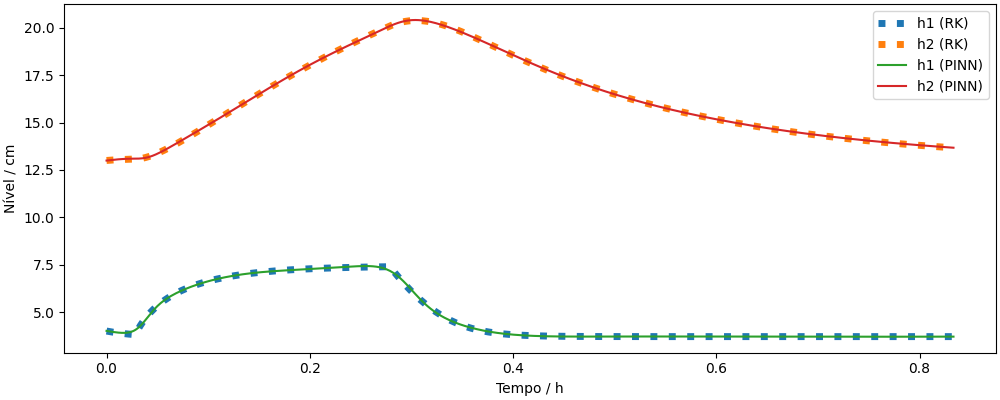
\includegraphics[width=1\textwidth]{pinn-result.png}
    \caption{Comparação entre as previsões da PINN e o método numérico (RK45).}
  \end{figure}
\end{frame}

\begin{frame}{Comparação de Tempos de Execução}
  \begin{figure}
    \centering
    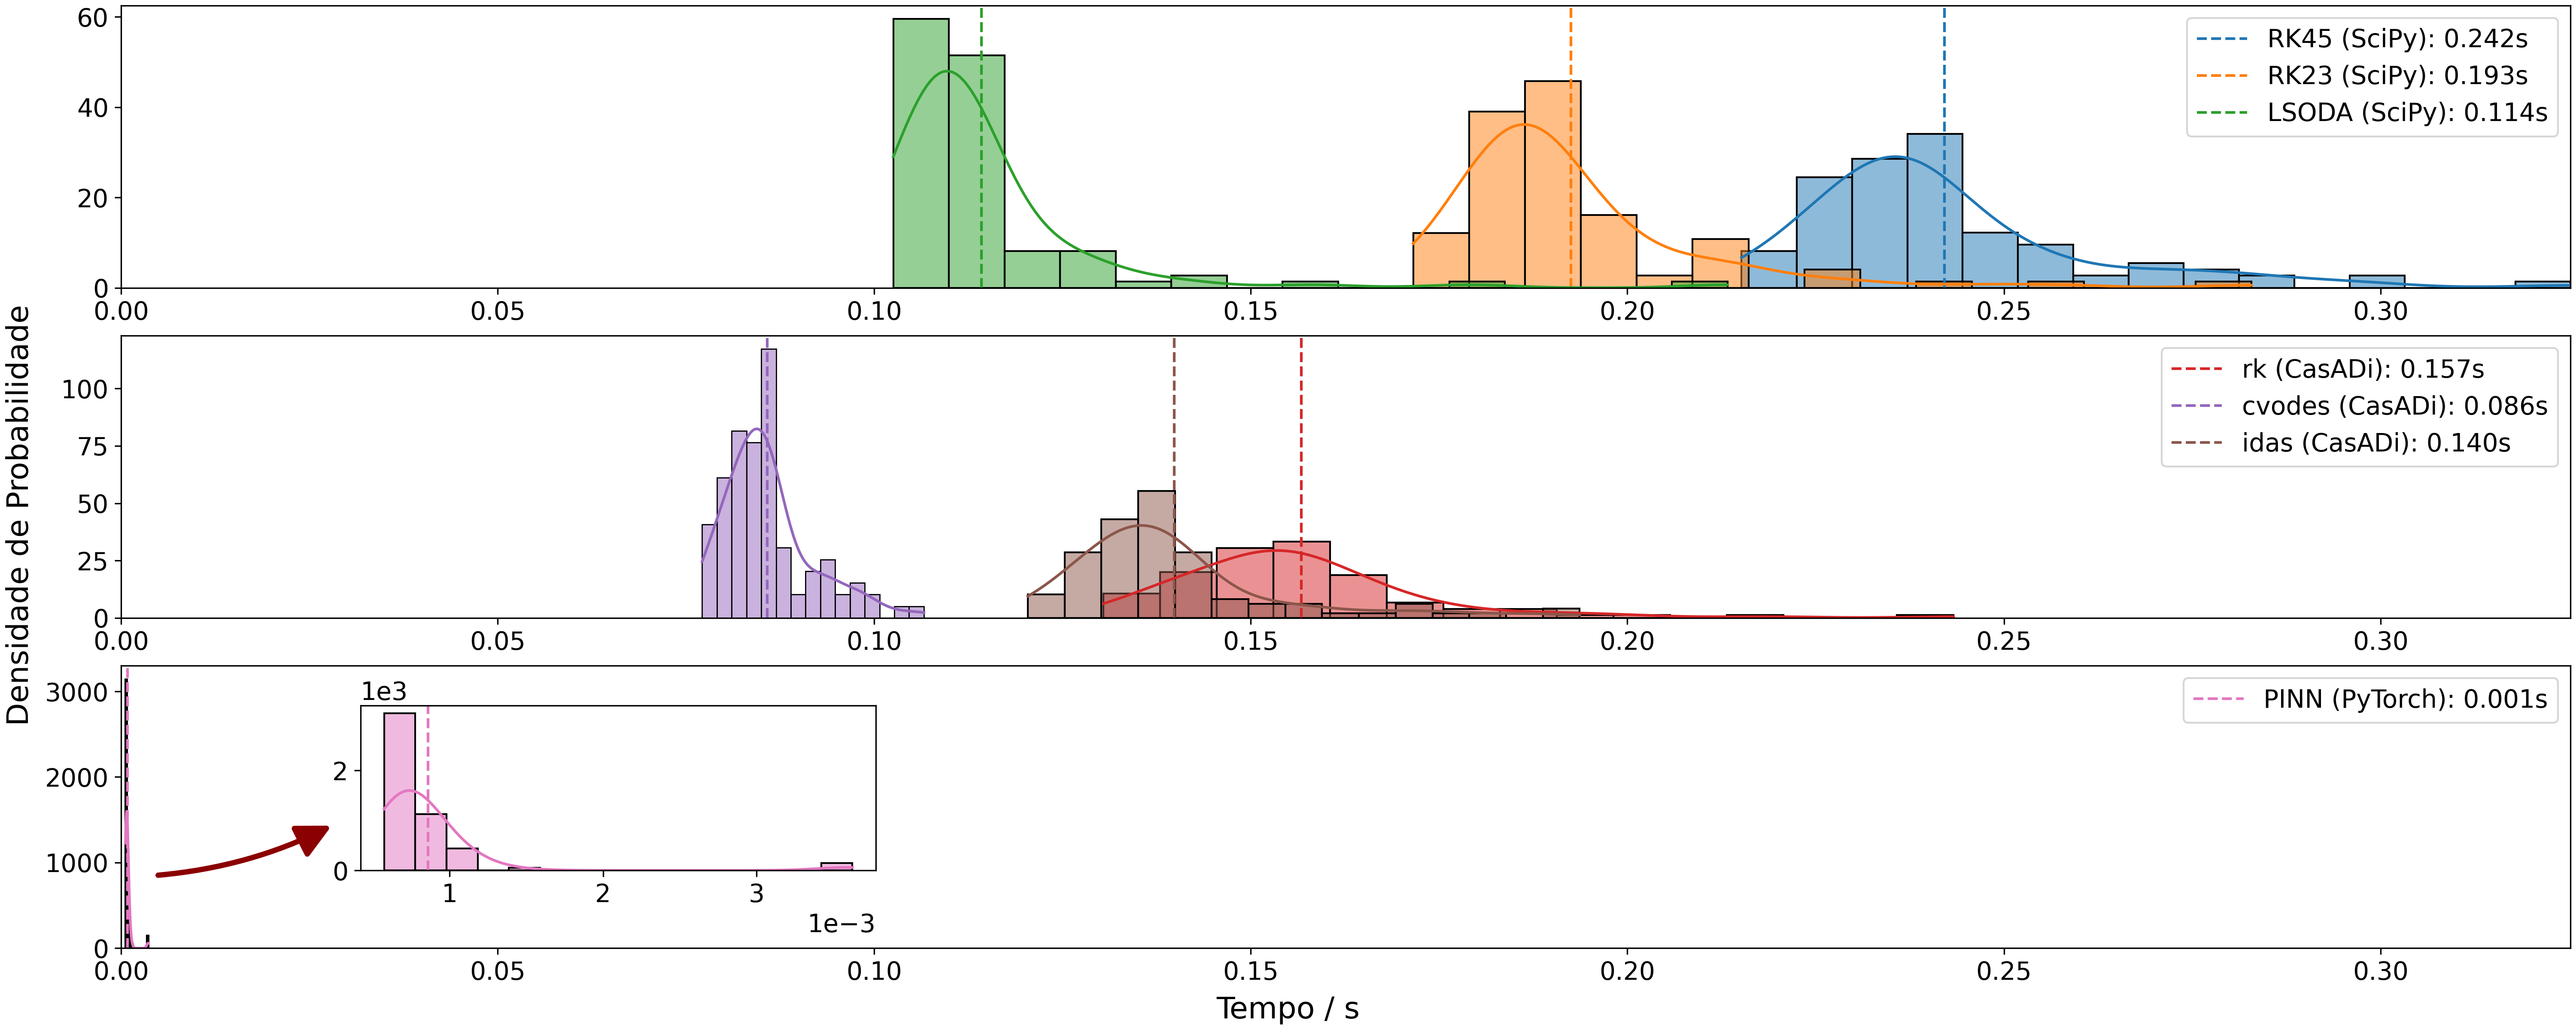
\includegraphics[width=\textwidth]{pinn-benchmark.png}
    \caption{Densidade de probabilidade dos tempos de execução dos métodos avaliados. Cada método foi executado 100 vezes; as linhas tracejadas indicam os tempos médios.}
  \end{figure}
\end{frame}

\section{A PIRNN (Physics-Informed Recurrent Neural Network)}

\begin{frame}{Introdução}
  \textbf{PIRNNs} incorporam memória recorrente e permitem uma modelagem mais precisa de sistemas dinâmicos \parencite{zheng_2023}.
  \\ \vspace{0.4cm}
  \begin{figure}
    \centering
    \begin{tikzpicture}[item/.style={circle,draw,thick,align=center},
    itemc/.style={item,on chain,join}]
  \begin{scope}[start chain=going right,nodes=itemc,every
    join/.style={-latex,very thick},local bounding box=chain]
    \path node (A0) {$A$} node (A1) {$A$} node (A2) {$A$} node[xshift=2em] (At)
    {$A$};
  \end{scope}
  \node[left=1em of chain,scale=2] (eq) {$=$};
  \node[left=2em of eq,item] (AL) {$A$};
  \path (AL.west) ++ (-1em,2em) coordinate (aux);
  \draw[very thick,-latex,rounded corners] (AL.east) -| ++ (1em,2em) -- (aux)
  |- (AL.west);
  \foreach \X in {0,1,2,t}
    {\draw[very thick,-latex] (A\X.north) -- ++ (0,2em)
      node[above,item,fill=gray!10] (h\X) {$\nu_\X$};
      \draw[very thick,latex-] (A\X.south) -- ++ (0,-2em)
      node[below,item,fill=gray!10] (x\X) {$x_\X$};}
  \draw[white,line width=0.8ex] (AL.north) -- ++ (0,1.9em);
  \draw[very thick,-latex] (AL.north) -- ++ (0,2em)
  node[above,item,fill=gray!10] {$\nu_t$};
  \draw[very thick,latex-] (AL.south) -- ++ (0,-2em)
  node[below,item,fill=gray!10] {$x_t$};
  \path (x2) -- (xt) node[midway,scale=2,font=\bfseries] {\dots};
\end{tikzpicture}

    \caption{Representação de uma RNN nas formas \textit{folded} e \textit{unfolded}. Fonte: Adaptado de Stack Exchange (2019)}
  \end{figure}
\end{frame}

\begin{frame}
  \textbf{Redes Neurais Recorrentes (RNNs)} usam o \textit{hidden state} ($\nu_t$) para alimentar o mesmo neurônio com as informações dos passos anteriores. Repetindo o processo até obter o estado oculto final \parencite{pytorch_2024}.
  \[
    \nu_t = \sigma(x_t \cdot W_{i\nu}^T + b_{i\nu} + \nu_{t-1} \cdot W_{\nu\nu}^T + b_{\nu\nu})
  \]
\end{frame}

\begin{frame}{Estrutura da PIRNN utilizada}
  A PIRNN utilizada consiste em 5 camadas, todas com a função de ativação tangente hiperbólica $(\tanh)$, com exceção da saída, que não possui função de ativação:

  \begin{itemize}
    \item Entrada: $\mathbf{X} = [[h_1^{(t-1)}, h_1^{(t)}], [h_2^{(t-1)}, h_2^{(t)}], [q^{(t-1)}, q^{(t)}]]$;
    \item \textcolor{red}{camada RNN: 32 neurônios;}
    \item camada linear 1: 32 neurônios;
    \item camada linear 2: 32 neurônios;
    \item camada linear 3: 32 neurônios;
    \item saída: $\mathbf{y} = [h_1^{(t+1)}, h_2^{(t+1)}]$.
  \end{itemize}

  Totalizando $32+32+32+32+2=130$ neurônios.
\end{frame}

\begin{frame}{A função \textit{loss} utilizada}
  A implementação da função \textit{loss} é um tanto diferente: agora não podemos usar a derivação automática, pois o tempo ($t$) não é uma entrada.

  Aqui, foi utilizada a derivada regressiva de 3 pontos (os 2 pontos fornecidos para a rede e o ponto previsto).

  \begin{equation}
    \mathcal{L} = w_1 \cdot \mathcal{L}_{\text{EDO}} + w_2 \cdot \mathcal{L}_{\text{data}}
  \end{equation}
  onde:
  \begin{itemize}
    \item $w_1, w_2$: pesos para o cálculo da Loss;
    \item $\mathcal{L}_{\text{EDO}}$: erro das equações diferenciais;
    \item $\mathcal{L}_{\text{data}}$: erro dos dados;
    \item $\mathcal{L}$: erro total.
  \end{itemize}
\end{frame}

\begin{frame}{Resultados}
  \begin{figure}
    \centering
    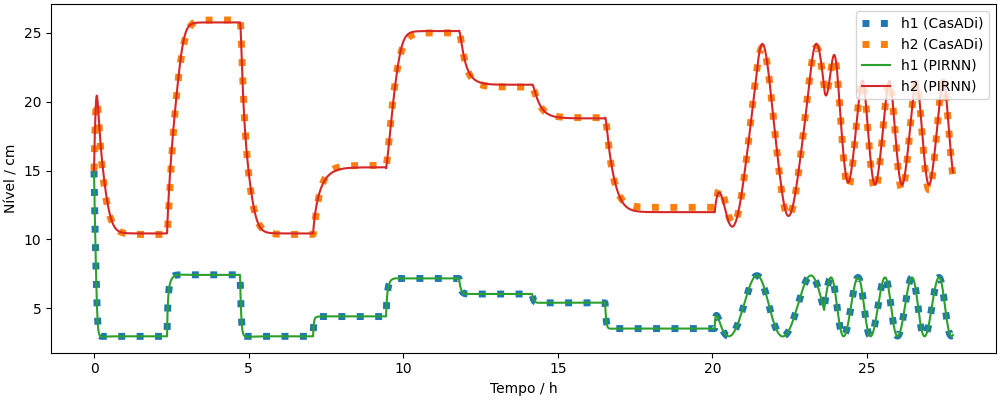
\includegraphics[width=1\textwidth]{pirnn-result.png}
    \caption{Comparação entre as previsões da PIRNN e o método numérico (RK)}
  \end{figure}
\end{frame}

\begin{frame}{Comparação de Tempos de Execução}
  \begin{figure}
    \centering
    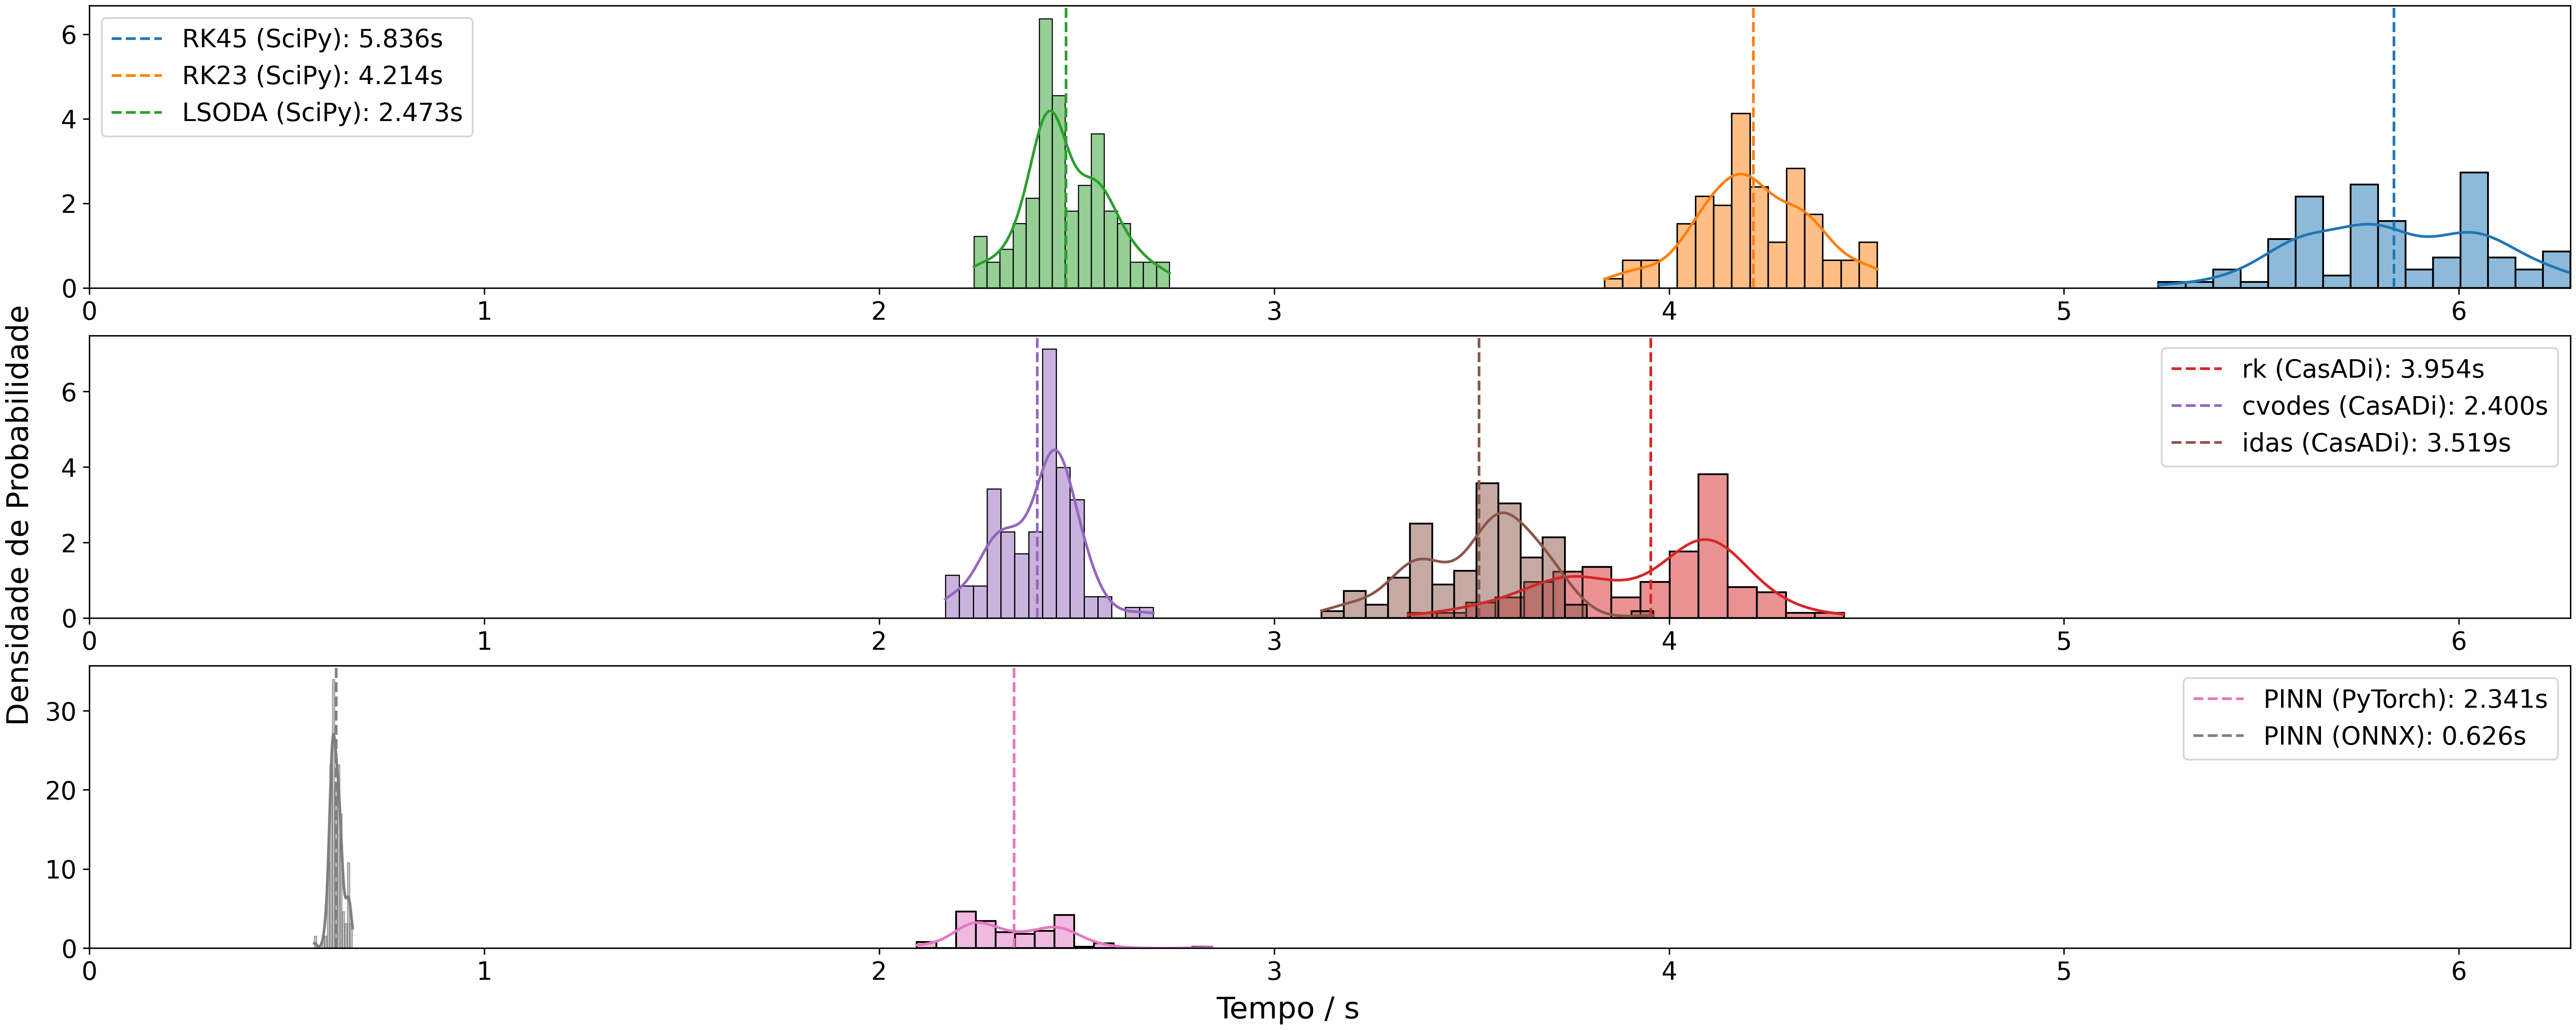
\includegraphics[width=\textwidth]{pirnn-benchmark.png}
    \caption{Densidade de probabilidade dos tempos de execução dos métodos avaliados. Cada método foi executado 100 vezes; as linhas tracejadas indicam os tempos médios.}
  \end{figure}
\end{frame}

\begin{frame}{Por que o ONNX Runtime é tão rápido?}
  \begin{columns}
    \begin{column}{0.5\textwidth}
      O ONNX Runtime é focado em desempenho de inferência e possui uma série de otimizações:
      \begin{itemize}
        \item ``constant folding'';
        \item ``redundant node eliminations'';
        \item ``node fusions''.
      \end{itemize}
    \end{column}
    \begin{column}{0.5\textwidth}
      \begin{figure}
        \centering
        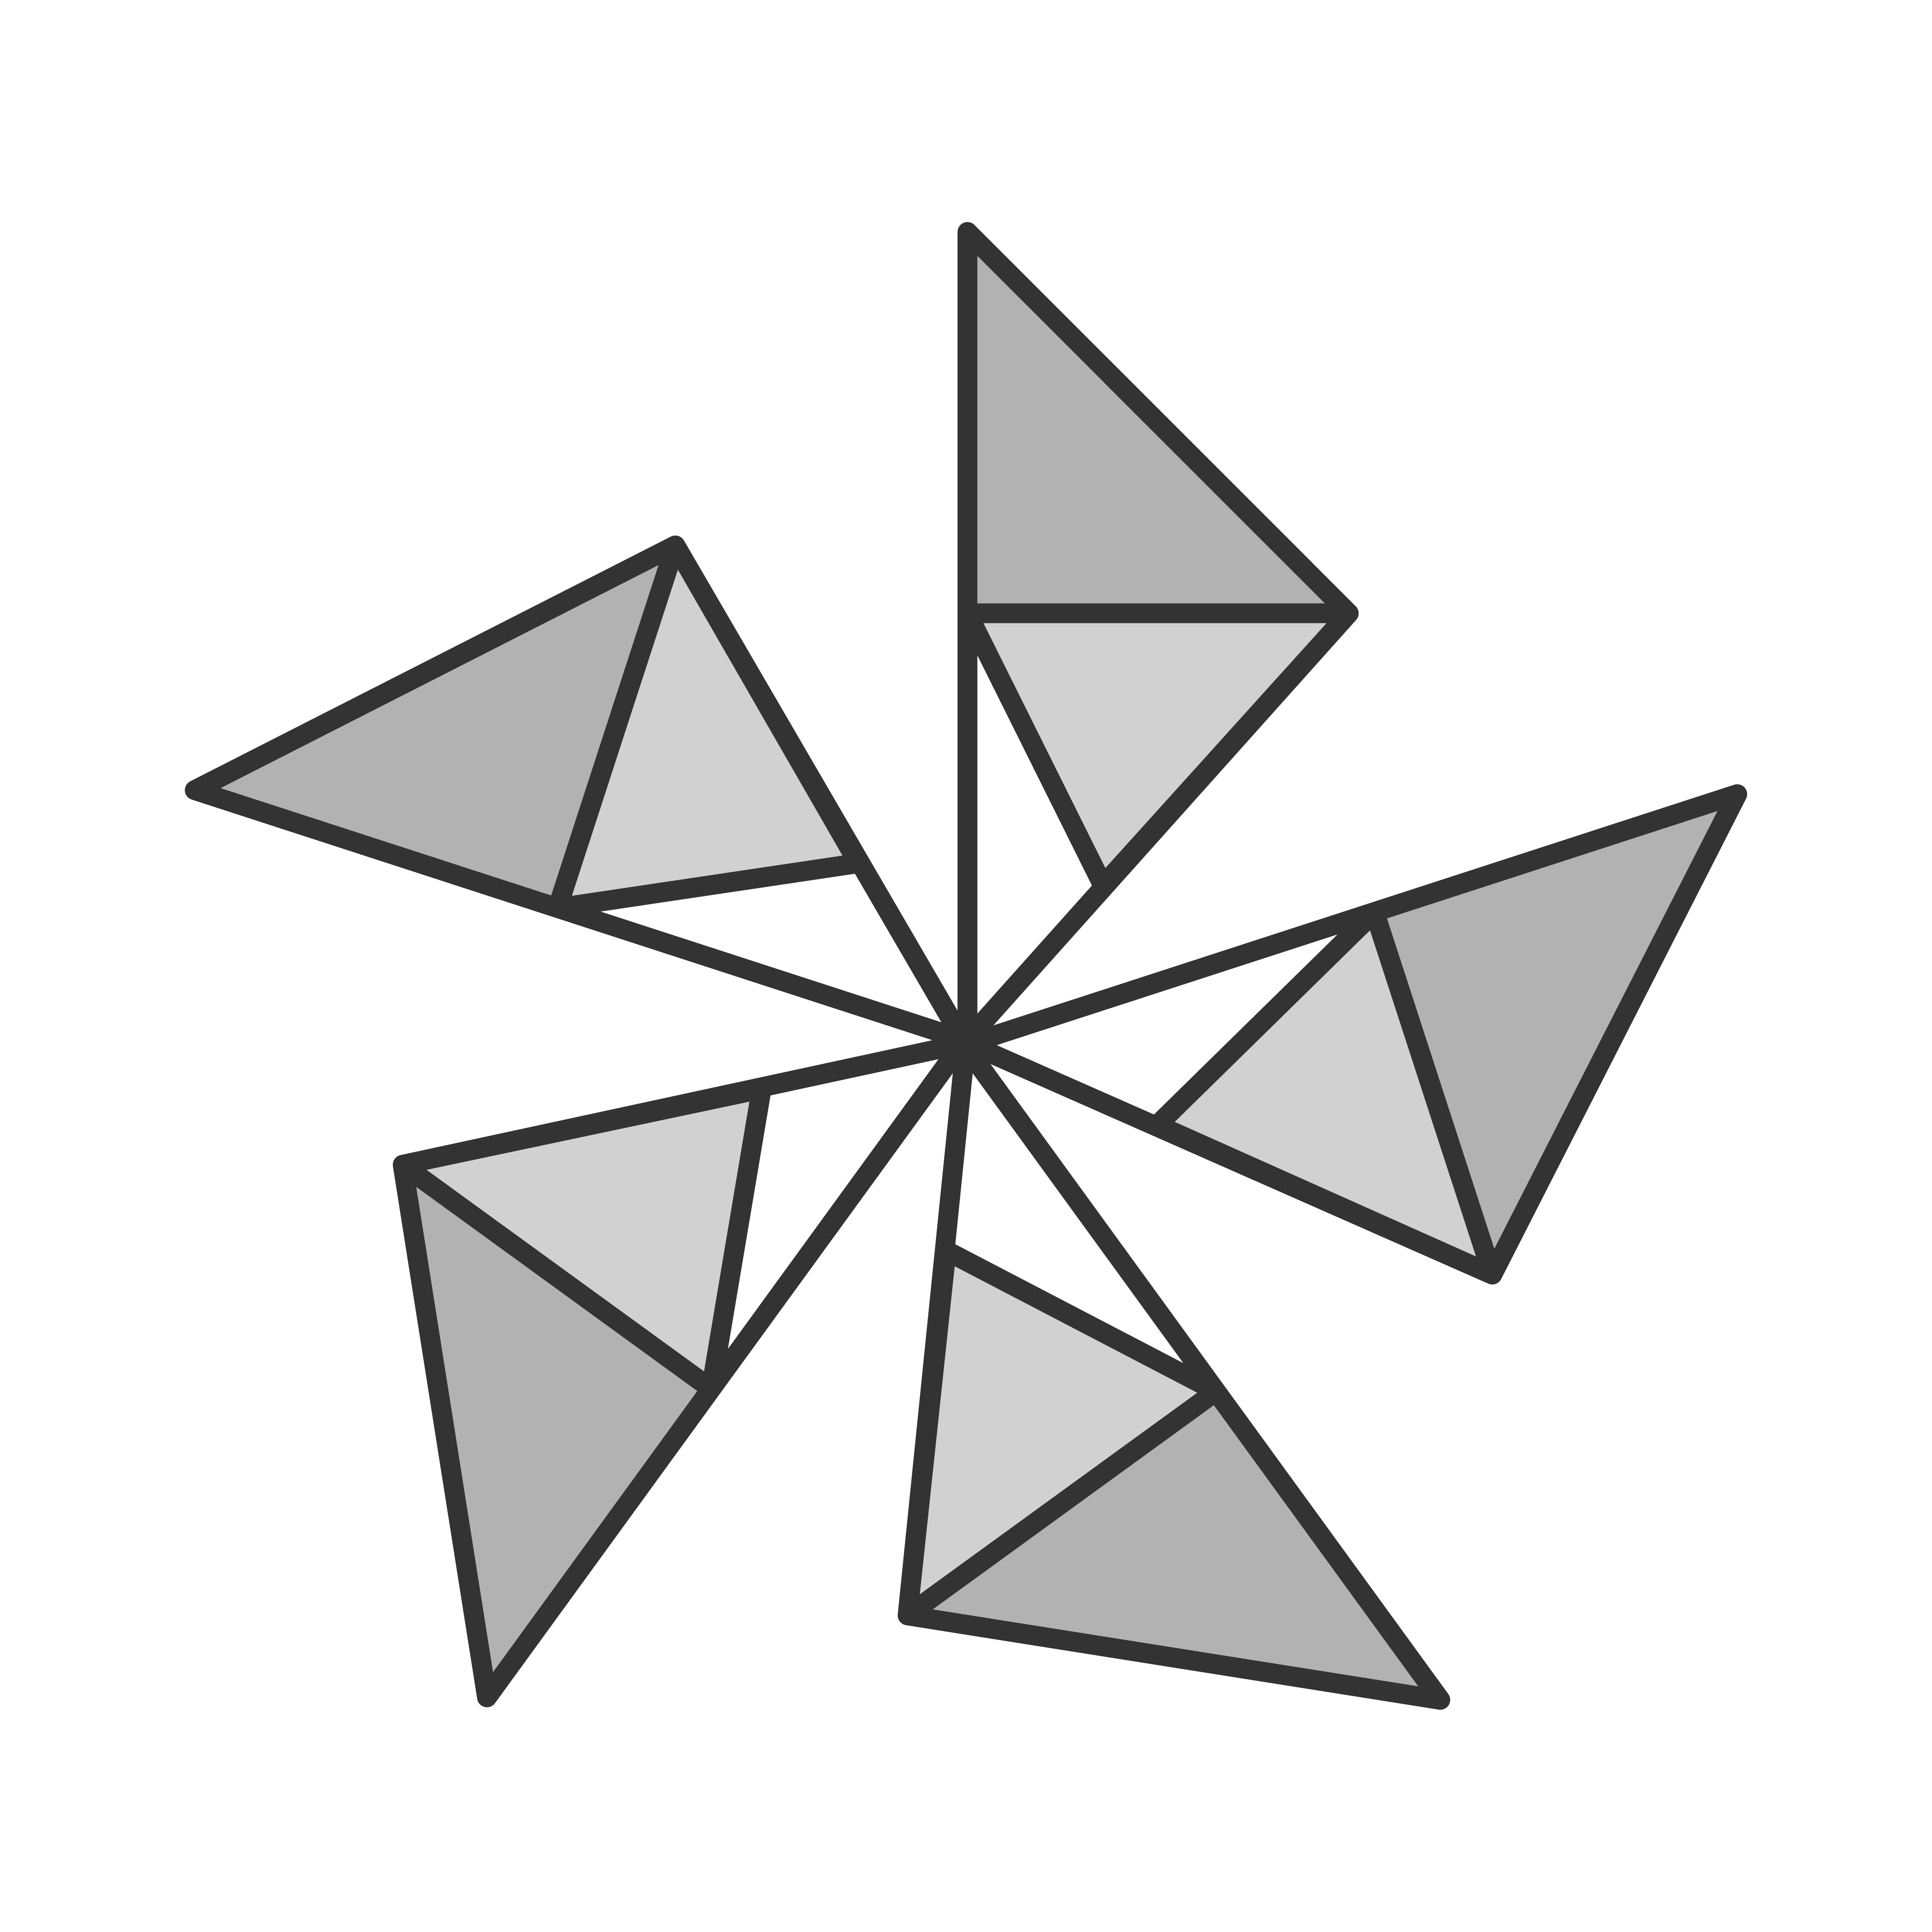
\includegraphics[width=4cm, keepaspectratio]{onnx.png}
        \caption{Logo do ONNX Runtime. Fonte: onnxruntime.ai (2017)}
      \end{figure}
    \end{column}
  \end{columns}
\end{frame}
\section{Implementação no Arduino}

\begin{frame}{O que é o Arduino?}
  \begin{columns}
    \column{0.6\textwidth}
    O Arduino é uma plataforma prototipagem amplamente utilizada por programadores devido ao seu baixo custo e facilidade para desenvolver \parencite{hughes_2016}. Entre as placas mais populares, destaca-se o Arduino UNO, a escolhida para esse trabalho.
    \begin{table}
      \centering
      \begin{tabular}{cc}
        \hline
        \textbf{Memória Flash} & \textbf{Memória RAM} \\ \hline
        32 kilobytes           & 2 kilobytes          \\ \hline
      \end{tabular}
      \caption{Memória disponível no Arduíno UNO.}
    \end{table}
    \column{0.4\textwidth}
    \begin{figure}
      \centering
      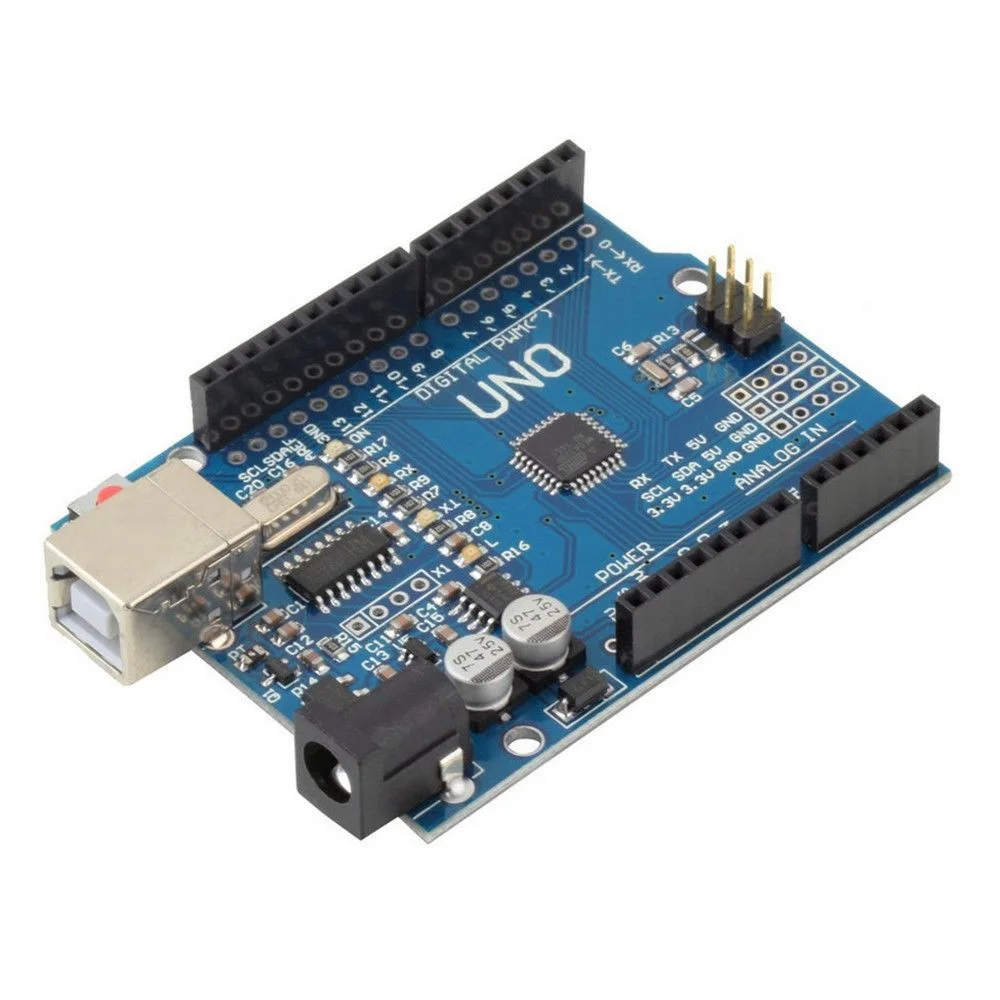
\includegraphics[width=\textwidth]{arduino.png}
      \caption{Placa Arduino UNO. Fonte: makerhero.com}
    \end{figure}
  \end{columns}
\end{frame}

\begin{frame}{O \textit{TankSim}}
  \begin{columns}
    \column{0.6\textwidth}
    \begin{figure}
      \centering
      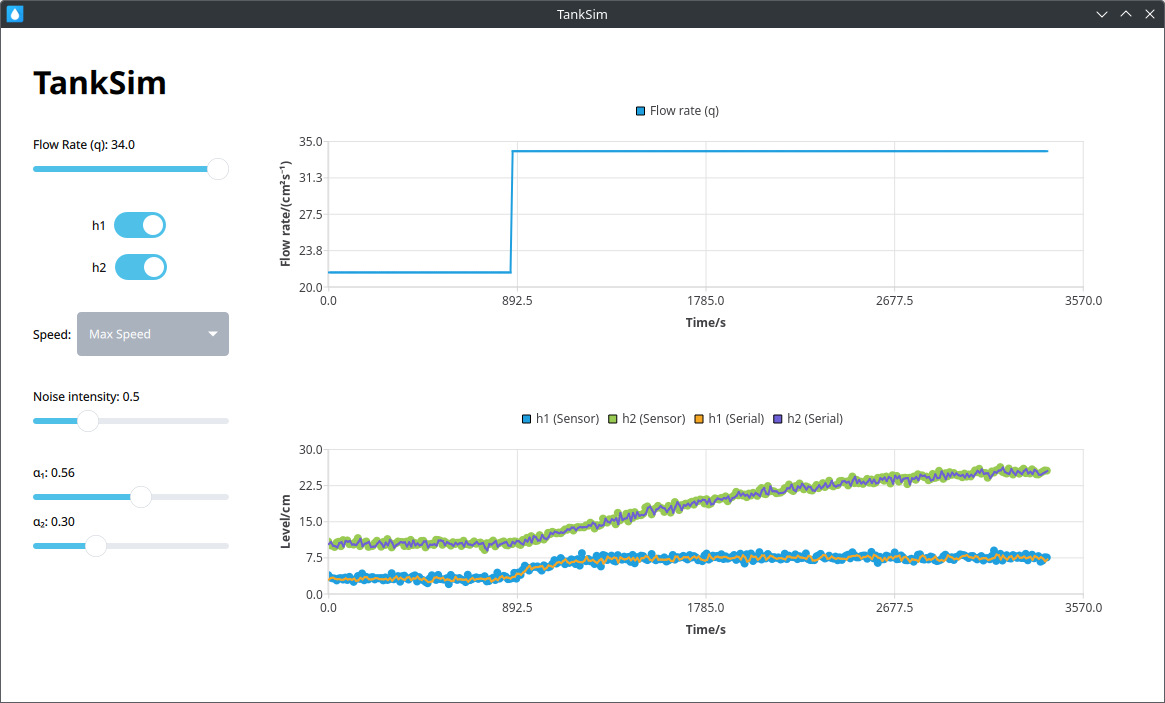
\includegraphics[width=\textwidth]{tanksim.png}
      \caption{Captura de tela do \textit{TankSim}.}
    \end{figure}

    \column{0.4\textwidth}
    O software \textit{TankSim} foi desenvolvido para:
    \begin{itemize}
      \item simular e manipular o funcionamento de uma planta;
      \item realizar a comunicação com o Arduino;
      \item visualizar os valores previstos pela rede neural;
    \end{itemize}
  \end{columns}
\end{frame}

\begin{frame}
  \begin{figure}
    \centering
    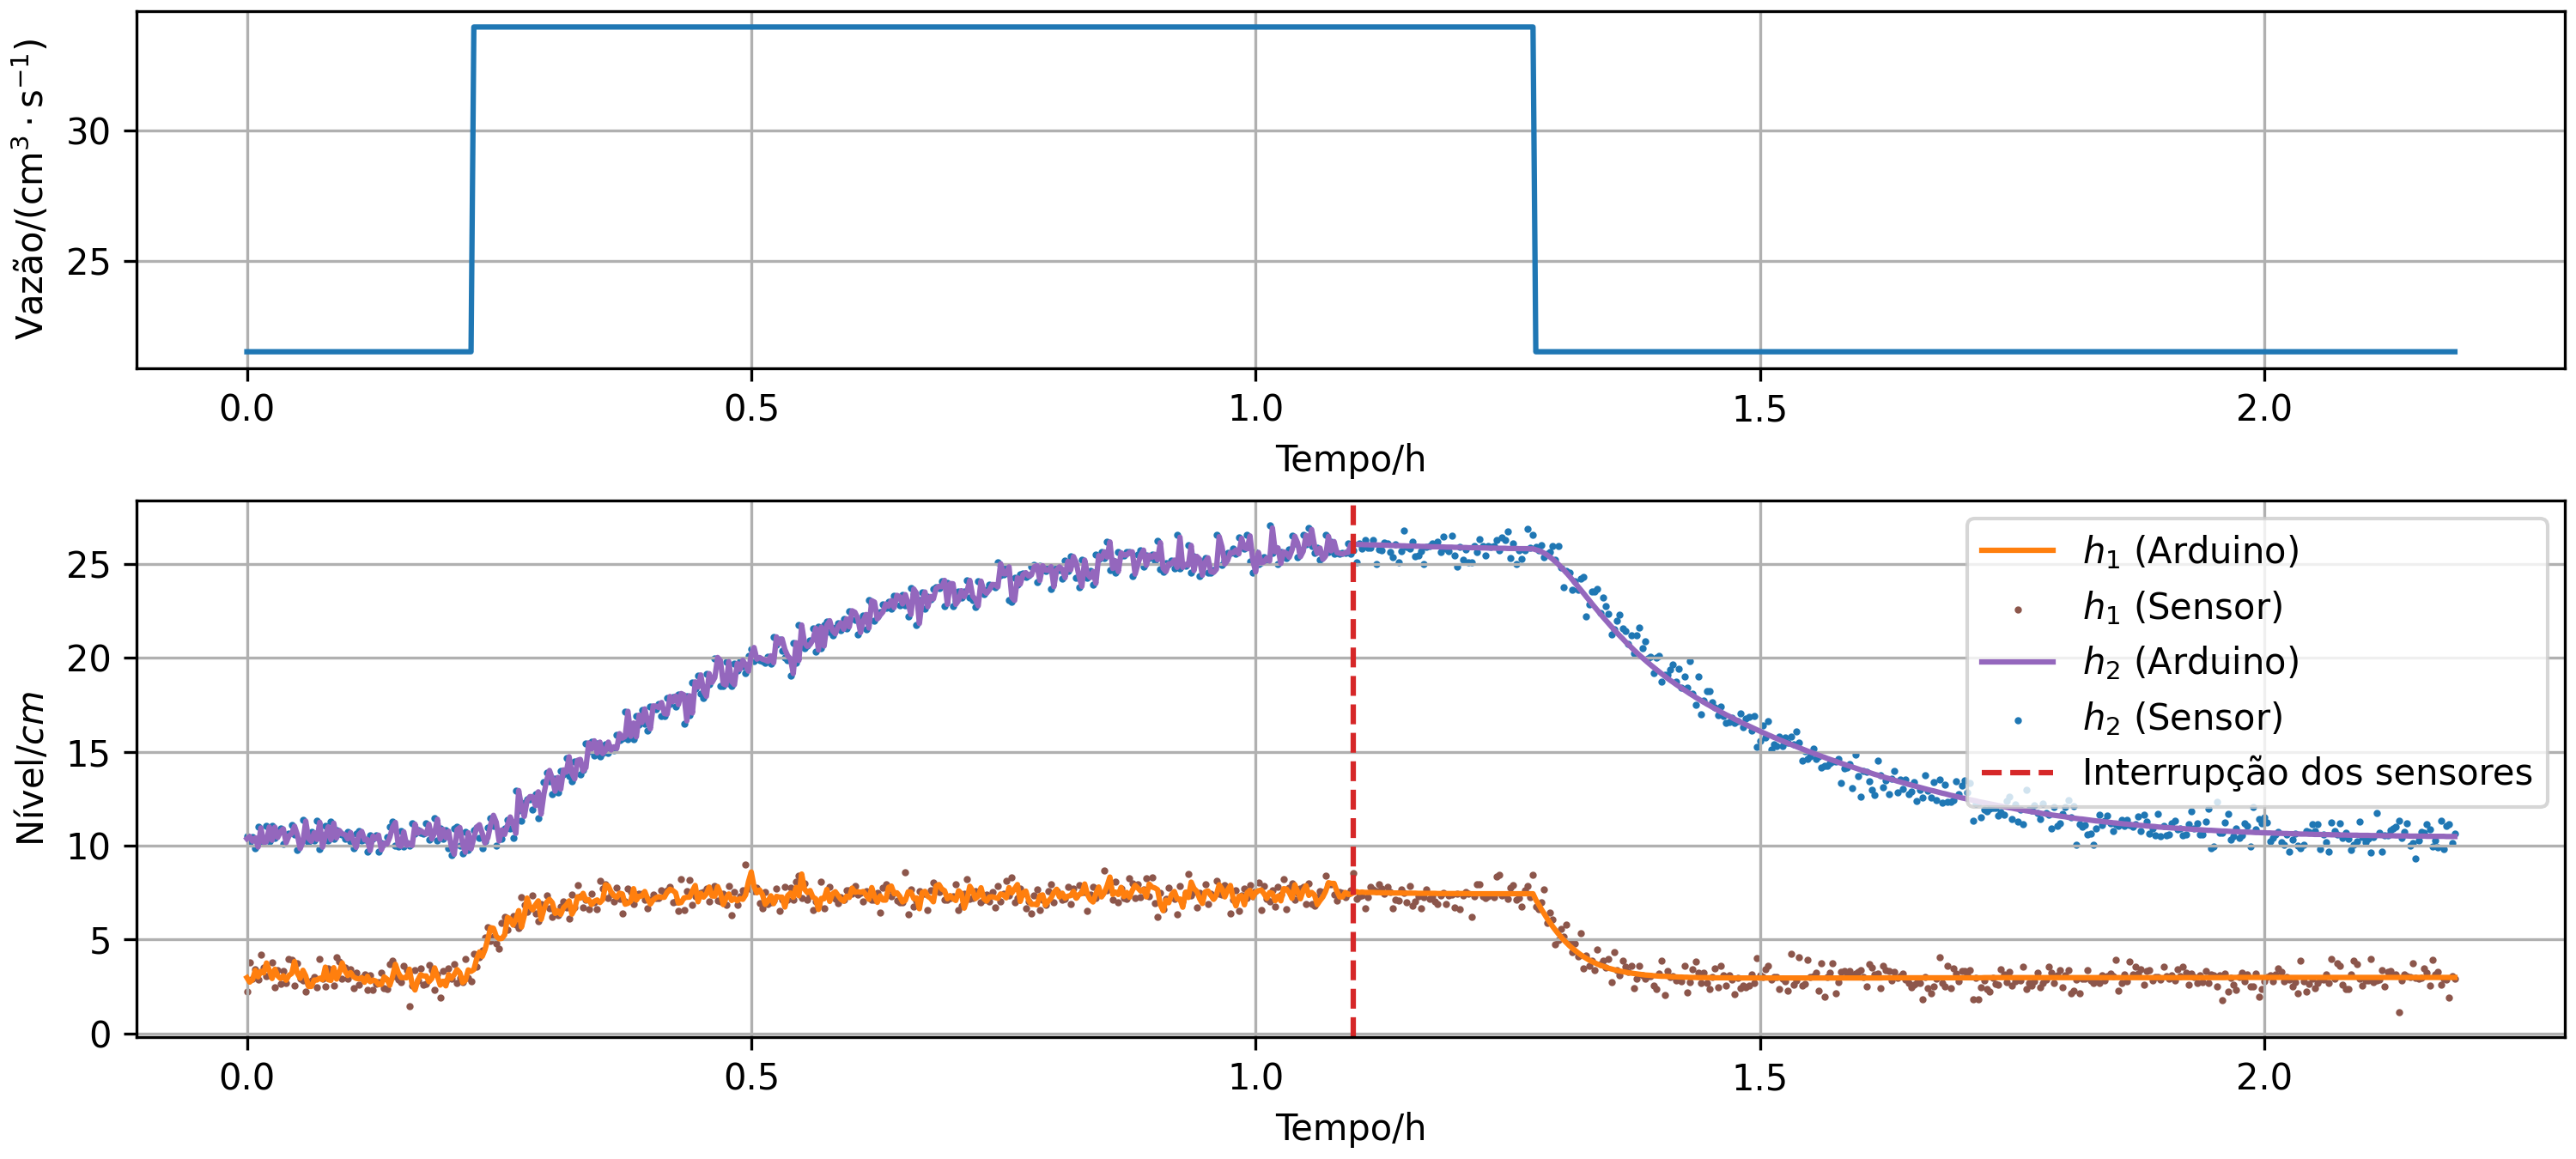
\includegraphics[width=0.9\textwidth]{sil-pirnn.png}
    \caption{Vazão de entrada $q_{\text{in}}$ e nível dos tanques $h_1$ e $h_2$, previstos pelo simulador e pela PIRNN embarcada no Arduino.}
  \end{figure}
\end{frame}
\section{Considerações finais}

Neste trabalho, foi demonstrada a utilização de uma PIRNN embarcada em um Arduino UNO para simular um sistema dinâmico formado por dois tanques esféricos em cascata. Os resultados mostraram que a PIRNN é uma alternativa viável aos métodos numéricos tradicionais e apresenta desempenho superior em relação ao tempo de simulação, sem grandes prejuízos a fidelidade das previsões. Isso a torna adequada para o controle em tempo real, sendo aplicável em automação industrial, monitoramento de processos e como analisador virtual. Sua compatibilidade com plataformas de baixo custo, como o Arduino, torna-a acessível e robusta, mantendo boa desempenho mesmo com falhas ou ruídos nas medições.

Contudo, em sistemas dinâmicos reais, é necessário considerar a degradação dos parâmetros do modelo ao longo do tempo, causada pelo desgaste ou envelhecimento dos componentes físicos. Essa degradação pode comprometer o desempenho da PIRNN, tornando necessário o retreinamento periódico do modelo para garantir sua acurácia. Nesse contexto, estudos futuros podem explorar técnicas de aprendizado por reforço, visando a adaptação em tempo real da PIRNN às mudanças dos parâmetros do sistema sem a necessidade de intervenções manuais.

Por fim, pesquisas adicionais podem investigar a implementação de modelos mais complexos, visando expandir a aplicabilidade das PIRNNs em sistemas dinâmicos descritos por equações diferenciais parciais.


{
  \logo{
    \raisebox{-1cm}{
      
\includegraphics[height=1cm, keepaspectratio]{anp.png}%
    }
    \hspace{4.4cm}
    \raisebox{-1cm}{
      
\includegraphics[height=1.4cm, keepaspectratio]{prh.png}%
    }
    \hspace{5.8cm}
    \raisebox{-1cm}{
      
\includegraphics[height=1.4cm, keepaspectratio]{brasao-ufba.png}%
    }
  }
  \begin{frame}{Agradecimentos}
    \centering \large Agradeço ao PRH 35.1 pelo suporte acadêmico e à Agência Nacional do Petróleo, Gás Natural e Biocombustíveis (ANP) pelo suporte financeiro e apoio ao desenvolvimento deste trabalho.
  \end{frame}
}

\begin{frame}[allowframebreaks]{Bibliografia}
  \printbibliography
\end{frame}

\end{document}